\ifx\wholebook\relax \else

\documentclass{article}
\usepackage[nomarginpar
  %, margin=.5in
]{geometry}

\addtolength{\oddsidemargin}{-0.05in}
\addtolength{\evensidemargin}{-0.05in}
\addtolength{\textwidth}{0.1in}

\usepackage[en]{../prelude}

\setcounter{page}{1}

\begin{document}

\title{Category Theory}

\author{Liu Xinyu
\thanks{{\bfseries Liu Xinyu} \newline
  Email: liuxinyu95@gmail.com \newline}
  }

\maketitle
\fi

\markboth{Category Theory}{Mathematics of Programming}

\ifx\wholebook\relax
\chapter{Category Theory}
\numberwithin{Exercise}{chapter}
\fi

\epigraph{Mathematics is the art of giving the same name to different things.}{--Henri Poincaré}

% Mathematics is the art of giving the same name to different things.

\begin{wrapfigure}{R}{0.4\textwidth}
 \centering
 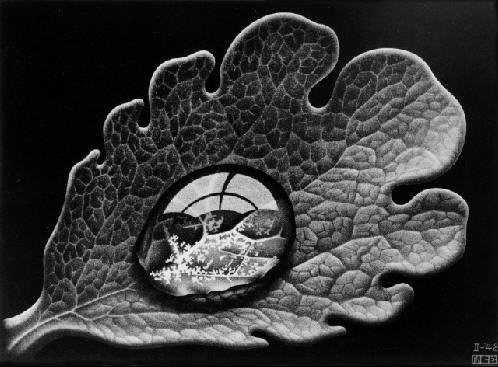
\includegraphics[scale=0.5]{img/dewdrop.eps}
 \captionsetup{labelformat=empty}
 \caption{Escher, Dewdrop, 1948}
 \label{fig:Escher-Dewdrop-1948}
\end{wrapfigure}

Welcome to the world of category! We just see the wounderful scence about abstract algebra in previous chapter. Congratulation to enter the door to the new kingdom of abstraction. The road to this kingdom is developed by may talent minds. In the first stage, people abstracted the concept of number and shape from the concrete things; in the second stage, we removed the meaning of numbers, shapes, and concrete arithmatics, abstract them to algebraic structures (for example group) and relations (for example isomorphism); category theory can be considered as the third stage.

What is category? Why does it matter? Any relationship between category and programming? Category theory was a `side product' when mathematicians studied homological algebra in 1940s. In recent decades, category theory has been widely used in varies of areas. Because of the powerful abstraction capability, it is applicable to many problem. It may also be used as an axiomatic foundation for mathematics, as an alternative to set theory and other proposed foundations. Category theory has practical applications in programming language theory. More and ore main stream programming laugnages adopted lambda calculus and closure. The usage of monads is relized in more than 20 languages\cite{Monad-Haskell-Wiki}. Speaking in the category language, a monad is a monoid in the category of endofunctors. Most of the foundamental computations have been abstracted in this way nowadays\footnote{For example, the traditional generic folding from right: \\
\texttt{foldr \_ z {[} {]} = z} \\
\texttt{foldr f z (x:xs) = f x (foldr f z xs)} \\
is written in category language as: \texttt{foldr f z t = appEndo (foldMap (Endo . f) t) z} We'll explain it later in this chapter.}.

The most important thing is abstraction. Hermann Weyl said ``"Our mathematics of the last few decades has wallowed in generalities and formalizations." The samething happens in programming. The problems in modern computer scients are challenging us with the complexicty we never seen before. Big-data, distributed, high concurrency, as well as the reuirement to consistency, security, and integrity. We can't catch them up in the traditional way, i.e. brute-force exhaustive search, pragmatic engineering practice, a smart idea plus some luck. It forces us to learn the new methods and tools from other sciences and mathematics.

As Dieudonne said: ``This abstraction which has accrued in no way sprang from a perverse desire among mathematicans to isolate themselves from the scientific community by the use of a hermetic language. Their task was to find solutions for problems {\em handed down by the `classical' age}, or arising directly from new discoveries in physics. They found that this was possible, but only through the {\em creation} of new objets and new methods, whose abstract character was {\em indispensable} to their success.'' \cite{Dieudonne1987}(page 2)

Category theory was developed by mathematician Samuel Eilenberg and Sauders Mac Lane in 1940s.

\begin{wrapfigure}{R}{0.3\textwidth}
 \centering
 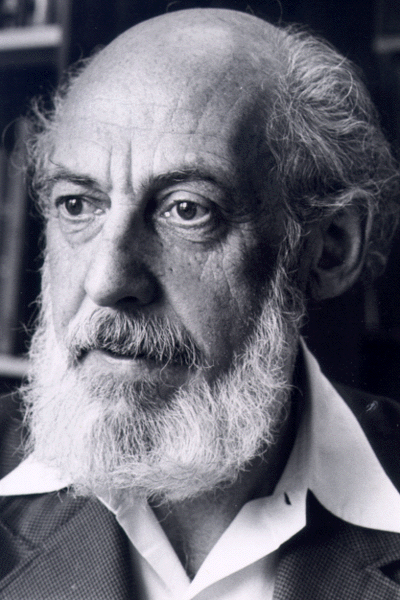
\includegraphics[scale=0.25]{img/Eilenberg.eps}
 \captionsetup{labelformat=empty}
 \caption{Samuel Eilenberg, 1913 - 1998}
 \label{fig:Eilenberg}
\end{wrapfigure}

\index{Samuel Eilenberg}
Samuel Eilenberg born in Warsaw, Kingdom of Poland to a Jewish family. His father is a brewer. Eilenberg studied at the University of Warsaw. A remarkable collection of mathematicians were on the staff there. He earned his Ph.D. from University of Warsaw in 1936. The second mathematical centre in Poland at that time was Lvov. It was there that Eilenberg met Banach, who led the Lvov mathematicians. He joined the community of mathematicians working and drinking in the Scottish Café and he contributed problems to the Scottish Book, the famous book in which the mathematicians working in the Café entered unsolved problems. In 1939 Eilenberg's father convinced him that the right course of action was to emigrate to the United States. Once there he went to Princeton. This was not too long in coming and, in 1940, he was appointed as an instructor at the University of Michigan. In 1949 André Weil was working at the University of Chicago and he contacted Eilenberg to ask him to collaborate on writing about homotopy groups and fibre spaces as part of the Bourbaki project. Eilenberg became a member of the Bourbaki team. He wrote the 1956 book {\em Homological Algebra} with Henri Cartan. Eilenberg mainly studied algebriac topology. He worked on the axiomatic treatment of homology theory with Norman Steenrod, and on homological algebra with Saunders Mac Lane. In the process, Eilenberg and Mac Lane created category theory. Eilenberg spent much of his career as a professor at Columbia University. Later in life he worked mainly in pure category theory, being one of the founders of the field. He was awarded Walf prize in 1987 for his fundamental work in algebraic topology and homological algebra. Eilenberg died in New York City during January 1998.

Eilenberg was also a prominent collector of Asian art. His collection mainly consisted of small sculptures and other artifacts from India, Indonesia, Nepal, Thailand, Cambodia, Sri Lanka and Central Asia. He donated more than 400 items to the Metropolitan Museum of Art in 1992\cite{Wiki-Eilenberg}.

\begin{wrapfigure}{L}{0.3\textwidth}
 \centering
 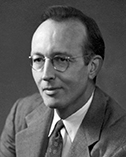
\includegraphics[scale=1]{img/Mac-Lane.eps}
 \captionsetup{labelformat=empty}
 \caption{Saunders Mac Lane, 1909 - 2005}
 \label{fig:Mac-Lane}
\end{wrapfigure}

\index{Saunders Mac Lane}
Saunders Mac Lane was born in Norwich, Connecticut in United State in 1909. He was christened "Leslie Saunders MacLane", but "Leslie" was later removed because his parents dislike it. He began inserting a space into his surname because his wife found it difficult to type the name without a space.

In high school, Mac Lane's favorite subject was chemistry. While in high school, his father died, and he came under his grandfather's care. His half-uncle helped to send him to Yale University, and paid his way there beginning in 1926. His mathematics teacher, Lester S. Hill, coached him for a local mathematics competition which he won, setting the direction for his future work. He studied mathematics and physics as a double major, and graduated from Yale with a B.A. in 1930. In 1929, at a party of Yale football supporters in New Jersey, Mac Lane was awarded a prize for having the best grade point average yet recorded at Yale. He met Robert Maynard Hutchins, the new president of the University of Chicago, who encouraged him to go there for his graduate studies\cite{Wiki-Mac-Lane}. Mac Lane Joined University of Chicago\footnote{Hutchins soon offered Mac Lane a scholarship after the party. But Mac Lane neglected to actually apply to the program, but showed up and was admitted anyway.}. At the University of Chicago he was influenced by Eliakim Moore, who was nearly seventy years old. He adviced Mac Lane to study for a doctorate at Göttingen in Germany certainly persuaded Mac Lane to work at the foremost mathematical research centre in the world at that time. In 1931, having earned his master's degree, Mac Lane earned a fellowship from the Institute of International Education and became one of the last Americans to study at the University of Göttingen prior to its decline under the Nazis.

At Göttingen, Mac Lane studied with Paul Bernays and Hermann Weyl. Before he finished his doctorate, Bernays had been forced to leave the university because he was Jewish, and Weyl became his main examiner. Mac Lane also studied with Gustav Herglotz and Emmy Noether. In 1934, he finished his doctor degree and returned to United State\footnote{Within days of finishing his degree, Mac Lane married Dorothy Jones, from Chicago, who had typed his thesis. It was a small ceremony followed by a wedding dinner with a couple of friends in the Rathaus Keller. The newly married couple quickly returned to the United States.}.

In 1944 and 1945, Mac Lane also directed Columbia University's Applied Mathematics Group, which was involved in the war effort. Mac Lane was vice president of the National Academy of Sciences and the American Philosophical Society, and president of the American Mathematical Society. While presiding over the Mathematical Association of America in the 1950s, he initiated its activities aimed at improving the teaching of modern mathematics. He was a member of the National Science Board, 1974–1980, advising the American government. In 1976, he led a delegation of mathematicians to China to study the conditions affecting mathematics there. Mac Lane was elected to the National Academy of Sciences in 1949, and received the National Medal of Science in 1989.

Mac Lann's early work was in field theory and valuation theory. In 1941, while giving a series of visiting lectures at the University of Michigan, he met Samuel Eilenberg and began what would become a fruitful collaboration on the interplay between algebra and topology. He and Eilenberg originated category theory in 1945.

Mac Lane died on April 14th, 2005 in San Francisco, California, USA.

\section{Category}

Let's use an example of ecosystem to understand category. There are varies of living species in African grassland, like lion, hyena, cheetah, antelope, buffalo, zebra, vulture, lizard, cobra, ant, ... We call these animals objects. Every type of animals and plants is an object. There are relation among these living things, for example, lion eats antelope, antelope eats grass. We can easily form a food chain by drawing an arrow from antelope to lion, and another arrow from grass to antelope. Hence these objects together with the arrows form a structured and connected system.

\begin{figure}[htbp]
 \centering
 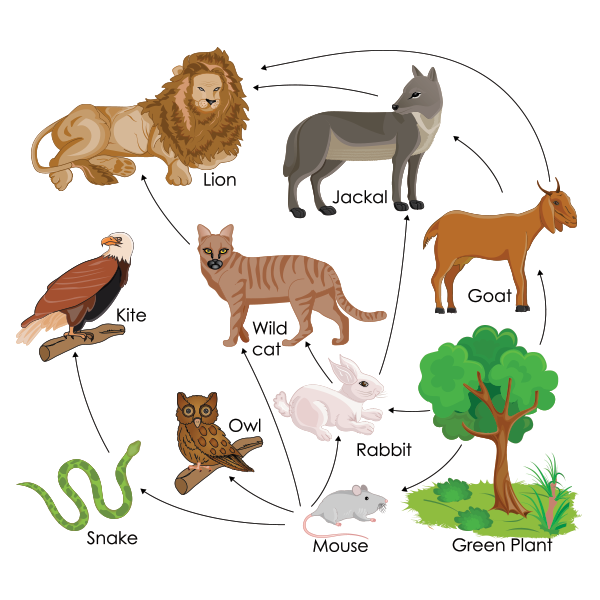
\includegraphics[scale=0.4]{img/food-chain.eps}
 %\captionsetup{labelformat=empty}
 \caption{Living objects and food chain arrows for a structured system}
 \label{fig:powerset}
\end{figure}

To become a category, this system has to satisfy two constraints. First, every object must have an arrow to itself. Such special arrow is called identity arrow. For the animals and plants in grassland, the arrow from lion to anteplope means the antelope is downstream to the lion in the foodchain. We can define that every species is downstream to itself along the foodchain (it does not mean one eat itself, but means one does not eat itself), hence every species has arrow points to itself. Second, arrows need be composible. What does composable mean? There is an arrow $f$ from grass to antelope, an arrow $g$ from antelope to lion. We can compose them to $g \circ f$, which means grass is downstream to lion along the food chain. This composed arrow can be further composed with the third one. For example, vulture eats the dead lion, thus we can draw an arrow $h$ from the lion to the volture. Composing them together gives $h \circ (g \circ f)$. This arrow means grass is downstream to vulture along the food chain. It is identical to the arrow $(h \circ g) \circ f$. Hence the upstream, downstream relations is associative.

Besides composable, there is another concept called commutative. As shown in below diagram:

\begin{center}
\begin{tikzpicture}
  \matrix (m) [matrix of math nodes,
               row sep=3em, column sep=4em, minimum width=2em]{
     & \text{Antelope} & \\
     \text{Grass} & & \text{Lion} \\};
  \path[-stealth]
    (m-2-1) edge node [above] {$f$} (m-1-2)
    (m-1-2) edge node [above] {$g$} (m-2-3)
    (m-2-1) edge node [below] {$h$} (m-2-3);
\end{tikzpicture}
\end{center}

There are two paths from grass to lion. One is the composite arrow $g \circ f$, which means grass is downstream to antelope, and antelope is downstream to lion; the other is arrow $h$, which means grass is downstream to lion. Hence we obtain a pair of parallel arrows:

\begin{center}
\begin{tikzpicture}
  \matrix (m) [matrix of math nodes,
               row sep=3em, column sep=4em, minimum width=2em]{
     \text{Grass} & \text{Lion} \\};
  \path[-stealth]
    (m-1-1.north east) edge node [above] {$g \circ f$} (m-1-2.north west)
    (m-1-1.south east) edge node [below] {$h$} (m-1-2.south west);
\end{tikzpicture}
\end{center}

These two arrow may or may note be the same, when they are, we say they are commutative:

\[
h = g \circ f
\]

And the grass, antelope, lion triangle commutes. We say the living things in the grassland form a category under the food chain arrows. It's time to give the formal definition for category.

\index{category} \index{arrow}
\begin{definition}
A category $\pmb{C}$ consists of a collection of objects\footnote{It has nothing related to the object oriented programming. Here the object means abstract thing.}, denoted as $A, B, C, ...$, and a collection of arrows, denoted as $f, g, h, ...$. There are four operations defined on top of them:
\begin{itemize}
\item Two total operations\footnote{Total operation is defined for every object without exception. its counterpart is partial operation, which is not defined from some objects. For example, the negate $x \mapsto -x$ is total operation for natural numbers, while the inverse operation $x \mapsto 1/x$ is not defined for 0, hence it is a partial operation.}, called source and target\footnote{They should be treated as verb, which means assign source object as... and assign target object as ...}. They assign source and target object to an arrow. Denoted as $A \arrowto{f} B$. It means the source of arrow $f$ is $A$, and the target is $B$;

\item The third total operation is called identity arrow\footnote{Similarly, identity arrow should be treated as verb, which means assign the identity arrow as...}. For every object $A$, the identity arrow points to $A$ itself. Denoted as $A \arrowto{id_A} A$;

\item The fourth operation is a partial operation, called composition. It composes two arrows. Given arrows $B \arrowto{f} C$ and $A \arrowto{g} B$, the composite of $f$ and $g$ is $f \circ g$, read as `$f$ after $g$'. It means $A \arrowto{f \circ g} C$.

\end{itemize}

Besides these four operations, category satisfies the following two axioms:

\begin{itemize}
\item \textbf{Associativity}: Arrows are associative. For every three composable arrows $f, g, h$, the equation:
\[
f \circ (g \circ h) = (f \circ g) \circ h
\]
holds. We can write it as $f\ g\ h$.
\item \textbf{Identity element}: The identity arrow is the identity element for the composition. For every arrow $A \arrowto{f} B$, equations:
\[
f \circ id_A = f = id_B \circ f
\]
hold.
\end{itemize}
\end{definition}

Categories and arrows are abstract compare to the food chain in grassland. Let's use some concrete examples to learn this definition.

\subsection{Examples of categories}

In mathematics, a set is called a monoid if it is defined with a special identity element, and associative binary operation. The integers for example, with 0 as the identity element, and plus as the binary operation, form a monoid called integer additive monoid.

A monoid can contains other things besides numbers. Consider the set of English words and sentences (called strings in programming). We can define the binary operation that concatenates two English strings. For example ``red'' $\doubleplus$ ``apple'' = ``red apple''. These English strings form a monoid, where the identity element is the empty string ``''. It's easy to verify the monoid constraints:

\[
red \doubleplus (apple \doubleplus tree) = (red \doubleplus apple) \doubleplus tree
\]

The string concatenation is associative.

\[
\texttt{""} \doubleplus apple = apple = apple \doubleplus \texttt{""}
\]

Concatenating any strings with empty string (identity element) gives itself.

Put the monoid of strings aside, let's consider another monoid. The elements are sets of characters. The binary operation is the set union; the identity element is the empty set. Union of two character sets gives a bigger set, for example:

\[
\{a, b, c, 1, 2\} \cup \{X, Y, Z, 0, 1\} = \{a, b, c, X, Y, Z, 0, 1, 2\}
\]

Plus the first example, the integer additive monoid, we have three monoids on hand. Let us setup the transforms among them\footnote{The transform is often called morphism in mathematics}. First is the map from monoid of English strings to monoid of character sets. For any given English word or sentence, we can collect all the unique characters used in it to form a set. Let's call this operation ``chars''. We can verify this operation satisfies the following:

\[
\begin{array}{rcl}
\text{chars}(red \doubleplus apple) = \text{chars}(red) \cup \text{chars}(apple) & \text{and} & \text{chars}(\texttt{""}) = \varnothing
\end{array}
\]

It means, the unique characters used in a concatenated English strings are same as the union result of the character sets for each one; empty string does not contain any characters (thus is an empty set).

Next, we define a transform from the monoid of character sets to integer additive monoid. For every given character set, we can count how many characters there are. Empty set contains 0 character. We can this operation ``count''

So far, we defined two transforms: ``chars'' and ``count'', let see how they composites:

\[
\text{String} \arrowto{\text{chars}} \text{Character set} \arrowto{\text{count}} \text{Integer}
\]

and

\[
\text{String} \arrowto{\text{count} \circ \text{chars}} \text{Integer}
\]

Obviously, the composite result ``count $\circ$ chars'' is also a transform. It means we first collect the unique characters from English strings, then count the number of characters. Hence we obtain the \text{monoid category} $\pmb{Mon}$. The objects are varies of monoids, arrows are the transforms among them, called morphisms in mathematics. The identity arrow is from a monoid to itself.

This is a very big category. It contains {\em all} the monoids in the universe\footnote{You may think about the Russel's paradox. Strictly speaking, $\pmb{Mon}$ contains all `small' monoid in the universe}. On the other hand, category can also be small. Let's see another example, a category that only contains only one monoid. Consider the monoid of English strings. There is only one object, which is the set of all English strings (I am sorry that this set does not look small). For any English string, for example `hello', we can define a prefix operation, that prepand `hello' to any other English strings. We call this operation as `prefix hello'. Apply `prefix hello' to word `Alice' gives result `helloAlice'; Similarly, we can define `prefix hi', when applied to `Alice' gives `hiAlice'. If we define them as two different arrows, then their composite arrow is:

\begin{center}
prefix hello $\circ$ prefix hi = prefix hellohi
\end{center}

It means first add prefix `hi', then add prefix `hello'. It easy to verify that, any three such arrows are associative. For the identity element, any string does not change when adding empty string as prefix, hence it is the identity arrow. Now we have a monoid category with only one object, as shown in figure \ref{fig:monoid-as-category}.

\begin{figure}[htbp]
\centering
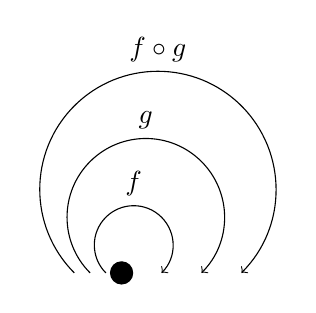
\begin{tikzpicture}
\filldraw (0, 0) circle (4pt) node (obj) {};
\draw[->] (-0.2, 0) arc[radius=5mm, start angle=225, end angle=-45] node[pos=0.5, above]{$f$};
\draw[->] (-0.4, 0) arc[radius=10mm, start angle=225, end angle=-45] node[pos=0.5, above]{$g$};
\draw[->] (-0.6, 0) arc[radius=15mm, start angle=225, end angle=-45] node[pos=0.5, above]{$f \circ g$};
\end{tikzpicture}
\caption{The monoid category with only one object}
\label{fig:monoid-as-category}
\end{figure}

\index{Monoid category}
For monoid, we see both the category $\pmb{Mon}$, that contains all the monoids in the universe, and the category with only one monoid. It is like a hidden world in a piece of sand. What's more interesting, for any object $A$ in a category $\pmb{C}$, define set $hom(A, A)$ as all the arrows from $A$ to $A$ itself. Then this set of arrows for a monoid under composite operation, where the identity element is the identity arrow. Such symmetry emerges surprisingly.

\index{Category of sets under total functions}
Our second example is set. Let every set be an object\footnote{Whenever consider the set of all sets, it ends up of Russel's paradox `the set all sets that does not contain itself'. We'll revisit Russel's paradox in chapter 7.}, the arrow is a function (or map) from one set $A$ to another set $B$. We call $A$ the domain of definition, and $B$ is the domain of the function value\footnote{It is total function, which can be applied to every elements in domain $A$.}. The composition is function composite. For functions $y = f(x)$ and $z = g(y)$, their composition is $z = (g \circ f)(x) = g(f(x))$. It's easy to verify that function composition is associative. The identity element is the identity function $id(x) = x$. Hence we obtain the category $\pmb{Set}$ of all sets and functions.

\index{partial order set} \index{poset}
\index{pre-order set} \index{preset}
Our third example contains a pair of concepts. {\em partial order set} and {\em pre-order set}. Given a set, pre-order means we can compare every two elements in it. We often use the symbol $\leq$ to represent this binary relation. It is not necessarily means less or greater than like numbers, it can mean one set is subset of the other, one string is post-fix of the other, one person is descendant of the other etc. If the relation $\leq$ satisfy the following conditions, we call it a pre-order:

\begin{itemize}
\item \textbf{reflexive}: For every element $a$ in the set, we have $a \leq a$;
\item \textbf{transitive}: If $a \leq b$ and $b \leq c$, then $a \leq c$;
\end{itemize}

On top of these two, if the relation is also anti-symmetric, we call it partial order:

\begin{itemize}
\item \textbf{anti-symmetric}: if $a \leq b$ and $b \leq a$, then $a = b$;
\end{itemize}

We define the set satisfies pre-oder preset, and the set satisfies partial order poset:

\[
preset \quad \quad \quad poset
\]

\begin{figure}[htbp]
\centering
\begin{tikzpicture}[scale=0.5]
  \matrix (m) [matrix of math nodes,
               row sep=1em, column sep=1em, minimum width=2em]{
     % 4 row x 6 column
     & \shortstack{Old ``Scotty'' \\ McDuck} & & & \shortstack{Grandma \\ Duck} & \\
     \shortstack{Scrooge \\ McDuck} & \shortstack{Matilda \\ McDuck} & \shortstack{Goosetail \\ Gander} & \shortstack{Hortense \\ McDuck} & \shortstack{Quackmore \\ Duck} & \shortstack{Daphne \\ Duck} \\
     & & \shortstack{Gladstone \\ Gander} & \shortstack{Donald \\ Duck} & \shortstack{Thelma \\ Duck} & \\
     & & & \text{Huey} & \text{Dewey} & \text{Louie} \\};
  \path[<-]
    (m-1-2) edge (m-2-1) % Scotty -- Scrooge
    (m-1-2) edge (m-2-2) % Scotty -- Matilda
    (m-1-2) edge (m-2-4) % Scotty -- Hortense
    (m-1-5) edge (m-2-5) % Grandma -- Quackmore
    (m-1-5) edge (m-2-6) % Grandma -- Daphne
    (m-2-3) edge (m-3-3) % Goosetail -- Gladstone
    (m-2-5) edge (m-3-4) % Quackmore -- Donald
    (m-2-5) edge (m-3-5) % Quackmore -- Thelma
    (m-3-5) edge (m-4-4) % Thelma -- Huey
    (m-3-5) edge (m-4-5) % Thelma -- Dewey
    (m-3-5) edge (m-4-6); % Thelma -- Louie
\end{tikzpicture}
\caption{Duck family tree}
\label{fig:genealogical-tree}
\end{figure}

Not every two elements are comparable in partial order set. The figures in Duck Donald family form a partial order set under the descendant relations, as shown in figure \ref{fig:genealogical-tree}. We can see Donald$\leq$Quackmore, but there is no $\leq$ relation between Huey and Donald, or between Donald and Scrooge. Although every one has its ancestor in this family tree (The figures at the root can be considered as the ancestor of themselves according to reflexive rule), but the figures at the same level or in different branches are not comparable.

As shown in \ref{fig:powerset}, for a given set $\{x, y, z\}$, all its subsets form a partial order set under the inclusion relationship. Although every element (a subset) has a subset, elements at the same level are not comparable. Besides that there are also non-comparable elements, like $\{x\}$ and $\{y, z\}$ for example.

\begin{figure}[htbp]
 \centering
 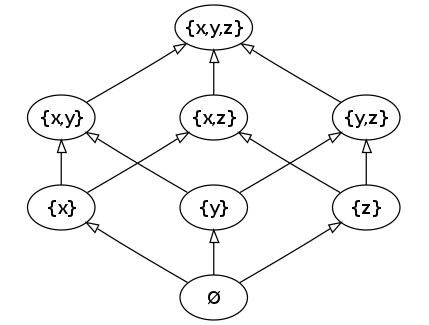
\includegraphics[scale=0.4]{img/powerset.eps}
 %\captionsetup{labelformat=empty}
 \caption{All subsets form a partial order set under inclusion relationship}
 \label{fig:powerset}
\end{figure}

\index{category of partial order set} \index{category of pre-order set}
In general any partial order set is a pre-order set, but the reverse is not necessarily true. A pre-order set may not be partial order set. We learn monotone function in high school math. Monotone function never decreases, if $x \leq y$, then $f(x) \leq f(y)$. By composing monotone functions on top of partial order set or pre-order set, we obtain a pair of categories.

\[
\pmb{Pre} \quad \quad \quad \pmb{Pos}
\]

The objects are all $presets$ and $posets$, the arrows are monotone maps. As the identity map is also monotone, it is the identity arrow in the category.

We intended choose categories of monoids and pre-set as two examples. They are the two most simple categories. The study of monoids is the study of composition in the miniature. The study of presets is the study of comparison in the miniature. It is the core of the entire category to study the composition and comparison of mathematical structures. In a sense every category is an amalgam of certain monoids and presets(\cite{Simmons2011}, p13).

$\pmb{Pre}$ is a big category that contains all the pre-order sets in the world. On the other hand, preset category can also be very small, that only contains one pre-order set. Consider the set of elements $i, j, k, ...$, if $i$ and $j$ are comparable, and $i \leq j$, we define

\[
i \longrightarrow j
\]

Hence for every tow objects, either there is no arrow between them, which means they are not comparable; or there exists one, which means there is $\leq$ relationship. In summary, there is at most one arrow between any two objects. We can verify that such arrows are composable, and for every element $i$, relation $i \leq i$ holds, hence there exists self-pointed arrow. Such preset itself forms a category. Again, we see the symmetry between preset and monoid categories. Monoid category contains only one object, but has many arrows; while preset category contains many objects, but has at most one arrow between objects.

\begin{Exercise}
\Question{Verify the monoid $(S, \cup, \varnothing)$ (the elements are sets, the binary operation is set union, the identity element is empty set) and $(N, +, 0)$ (elements are natural numbers, the binary operation is add, the identity element is zero) are all categories that contain only one object.}
\Question{We introduced Piano's axioms for natural numbers in chapter 1, as well as the isomorphic structures to Piano arithmetic, like the linked-list etc. They can be described in categories. This was found by German mathematician Richard Dedekind although the category theory was not established by his time. We named this category as Piano category, denoted as $\pmb{Pno}$. The objects in this category is $(A, f, z)$, where $A$ is a set, for example natural numbers $N$; $f: A \to A$ is a successor function. It is $succ$ for natural numbers; $z \in A$ is the starting element, it is zero for natural numbers. Given any two Piano object $(A, f, z)$ and $(B, g, c)$, define the morphism from $A$ to $B$ as:

\[
A \arrowto{\phi} B
\]

It satisfies:

\[
\phi \circ f = g \circ \phi \quad \text{and} \quad \phi(z) = c
\]

Verify that $\pmb{Pno}$ is a category.}
\end{Exercise}

\subsection{Arrow $\neq$ function}

In most examples so far, arrows are either functions, or function like things, such as maps or morphisms. It gives us an illusion that arrow means function like things. The next example helps us to realize such deception. There is a relation category. The objects are sets. The arrow from set $A$ to set $B$, $A \arrowto{R} B$ is defined as:

\[
R \subseteq B \times A
\]

Let's see what does it mean. Set $B \times A$ represents all element combinations from $B$ and $A$. It is called the product of $B$ and $A$:

\[
B \times A = \{(b, a) | b \in B, a \in A\}
\]

Use the Donald Duck family for example, set $A =$ \{ Scrooge McDuck, Matilda McDuck, Hortense McDuck\} contains three members in McDuck family, set $B = $ \{Goosetail Gander, Quackmore Duck\} contains two external members, then the product of $B \times A$ is \{(Goosetail Gander, Scrooge McDuck),(Goosetail Gander, Matilda McDuck), (Goosetail Gander, Hortense McDuck), (Quackmore Duck, Scrooge McDuck), (Quackmore Duck, Matilda McDuck), (Quackmore Duck, Hortense MuDuck)\}. Set $R$ is a subset of $B \times A$, it represents some relation between $A$ and $B$. If element $a$ in $A$, and element $b$ in $B$ satisfy relation $R$, then $(b, a) \in R$, we denote it as $bRa$. For this example, we can let $R=$ \{(Goosetail Gander, Matilda McDuck), (Quackmore Duck, Hortense MuDuck)\}, then $R$ means they are couples (In Donald Duck story, Goosetail married Matilda, they adopted Gladstone as their child; Quackmore married Hortense, they are parent of Donald).

Hence the set of {\em all} arrows from $A$ to $B$ represents all possible relations from $A$ to $B$. Let's consider the arrow composition:

\[
A \to B \to C
\]

If there exists an element $b$ in some intermediate set, that both relations $bRa$ and $cSb$ hold, we say there is composition between arrows. Use the Donald Duck family for example. Let set $C=$ = \{Gladstone, Donald, Thelma\}. Relation $S=$ \{(Donald, Quackmore), (Thelma, Quackmore)\} means son and father. Thus the composite arrow $S \circ R$ gives result \{(Donald, Hortense), (Thelma, Hortense)\}, it means the relation $c$ is son of mother $a$. Hence both relations are satisfied through Quackmore, so that Donald and Thelma are sons of their mother Hortense. The definition of identity arrow is simple, every element has a identical relation to itself.

We can generate a new category from any existing category, for example, by reversing the arrows in category $\pmb{C}$, we obtained a dual {\em opposite} category $\pmb{C}^{op}$. Hence when we understand a category, we understand its dual category as well.

\section{Functors}

We mentioned category theory is the `second' level abstraction on top of algebraic structure. We've seen how to abstract all sets and maps, groups and morphisms, posets and monotone functions into categories. The next question is how to bridge these categories and compare them? Functor\footnote{Some C++ programming language materials use functor to name function object. It has nothing related to category theory.} is used to compare categories and their inner relations (objects and arrows).

\subsection{Definition of functor}
\index{函子}
In some sense, functor can be considered as the transform (morphism) between categories. However, it does not only map the object from one category to the other, but also maps the arrow. This makes functor different from the normal morphism (between groups for example).

We often use $\mathbf{F}$ to denote functor. Since functor likes the morphisms for category, it must faithfully preserve the structure and relations between categories. In order to achieve this, a functor need satisfy two conditions:

\begin{itemize}
\item The first condition. Any identity arrow in one category is transformed to identity arrow in another category. As shown in below figure:

\[
A \arrowto{id} A \quad \longmapsto \quad \mathbf{F}A \arrowto{id} \mathbf{F}A
\]

\index{covariance} \index{contravariance}
\item The second condition. Any composition of arrows in one category is transformed to composition in another category\footnote{There are two different types of transformation, one is called covariance, the other is contravariance. The two terms are also used in programming language type system. We only considered covariance in this book}.

\begin{center}
\begin{tikzpicture}
  \matrix (m) [matrix of math nodes,
               row sep=2em, column sep=2.5em, minimum width=2em]{
       & B &   & \longmapsto &             & \mathbf{F}B & \\
     A &   & C & \text{covariance} & \mathbf{F}A &  & \mathbf{F}C\\};
  \path[-stealth]
    (m-2-1) edge node [above] {$f$} (m-1-2)
    (m-1-2) edge node [above] {$g$} (m-2-3)
    (m-2-1) edge node [below] {$g \circ f$} (m-2-3)
    (m-2-5) edge node [above] {$\mathbf{F}(f)$} (m-1-6)
    (m-1-6) edge node [above] {$\mathbf{F}(g)$} (m-2-7)
    (m-2-5) edge node [below] {$\mathbf{F}(g \circ f)$} (m-2-7);
\end{tikzpicture}
\end{center}

\[
\mathbf{F}(g \circ f) = \mathbf{F}(g) \circ \mathbf{F}(f)
\]
\end{itemize}

In summary, functor preserve identity morphisms and composition of morphisms. Functors can also be composited, for example functor $(\mathbf{F} \mathbf{G})(f)$ means first apply $\mathbf{G}$ on arrow $f$, then apply $mathbf{F}$ on top of the arrow in the new category.

\subsection{Functor examples}
\label{sec:functor:examples}

\begin{wrapfigure}{R}{0.3\textwidth}
 \centering
 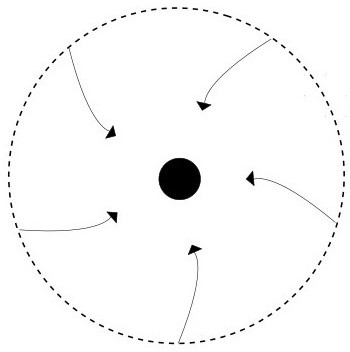
\includegraphics[scale=0.3]{img/blackhole.eps}
 \captionsetup{labelformat=empty}
 \caption{Constant functor acts like a blackhole.}
 \label{fig:blackhole}
\end{wrapfigure}

\index{functor!identity functor} \index{functor!id functor}
Let's use some examples to understand functor. If a functor maps a category to itself, it is called {\em endo-functor}\footnote{Similar to the automorphism in abstract algebra, which we introduced in previous chapter.}. The most simple functor is the identity functor, which is an endo-functor, denoted as $id: \pmb{C} \to \pmb{C}$. It can be applied to any category, maps object $A$ to $A$, and maps arrow $f$ to $f$.

\index{functor!constant functor}
The second simple functor is the constant functor. It acts like a blackhole. We denote it as $\mathbf{K}_B : \pmb{C} \to \pmb{B}$. It can be applied to any category, maps all objects to the blackhole object $B$, and maps all arrows to the identity arrow in the blackhole $id_B$. The blackhole category has only one identity arrow, it also satisfy the arrow composition condition: $id_B \circ id_B = id_B$.

\begin{example}
\normalfont
\index{functor!maybe functor}
Maybe functor. Computer scientist, Tony Hoare (Sir Charles Antony Richard Hoare), who developed the quicksort algorithm, and awarded ACM Turing award in 1980, had an interesting speaking apologised for inventing the null reference\footnote{At a software conference called QCon London in 2009}.

%\begin{wrapfigure}{L}{0.25\textwidth}
\begin{figure}[htbp]
 \centering
 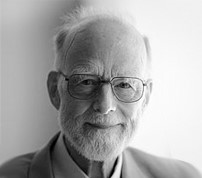
\includegraphics[scale=1]{img/Hoare.eps}
 \captionsetup{labelformat=empty}
 \caption{Tony Hoare}
 \label{fig:Hoare}
\end{figure}
%\end{wrapfigure}

\begin{quotation}
\itshape
I call it my billion-dollar mistake. It was the invention of the null reference in 1965. At that time, I was designing the first comprehensive type system for references in an object oriented language (ALGOL W). My goal was to ensure that all use of references should be absolutely safe, with checking performed automatically by the compiler. But I couldn't resist the temptation to put in a null reference, simply because it was so easy to implement. This has led to innumerable errors, vulnerabilities, and system crashes, which have probably caused a billion dollars of pain and damage in the last forty years\cite{Wiki-Hoare}.
\end{quotation}

After 2015, the main stream programming environments gradually adopted the maybe concept to replace the error prone null\footnote{For example the \texttt{Optional<T>} in Java and C++}.

Below diagram illustrates how $\mathbf{Maybe}$ behaves.

\begin{center}
\begin{tikzpicture}
  \matrix (m) [matrix of math nodes,
               row sep=2em, column sep=2.5em, minimum width=2em]{
     A & \mathbf{Maybe}\ A \\
     B & \mathbf{Maybe}\ B \\};
  \path[-stealth]
    (m-1-1) edge (m-1-2)
    (m-2-1) edge (m-2-2)
    (m-1-1) edge node [left] {$f$} (m-2-1)
    (m-1-2) edge node [right] {$\mathbf{Maybe}(f)$} (m-2-2);
\end{tikzpicture}
\end{center}

The left side objects $A$ and $B$ can be data types, like integer, Boolean. While the right side objects are mapped types through functor $\mathbf{Maybe}$. If $A$ represents $Int$, then the right side corresponds to $\mathbf{Maybe}\ Int$, if $B$ represents $Bool$, then the right side corresponds to $\mathbf{Maybe}\ Bool$. How does the maybe functor maps objects? that part is defined as this:

\lstset{frame=none}
\begin{lstlisting}
data Maybe A = Nothing | Just A
\end{lstlisting}

It means, if the object is type $A$, then the mapped object is type $\mathbf{Maybe}\ A$. Note the object is type, but not value. The value of $\mathbf{Maybe}\ A$ is either empty, denoted as $Nothing$, or a value constructed by $Just$.

Use type $Int$ for example, through the maybe functor, it is mapped to $\mathbf{Maybe}\ Int$. The value could be $Nothing$ or $Just\ 5$ for instance.

Consider a binary search tree, that contains elements of type $A$. When search a value in the tree, it may not be found, therefore the type of search result is $\mathbf{Maybe}\ A$\footnote{The complete example program can be found in the appendix of this chapter}.

\[
\begin{array}{rcl}
lookup\ Nil\ \_ & = & Nothing \\
lookup\ (Br\ l\ k\ r)\ x & = & \begin{cases}
  x < k: & lookup\ l\ x \\
  x > k: & lookup\ r\ x \\
  x = k: & Just\ k
\end{cases}
\end{array}
\]

For $\mathbf{Maybe}$ type data, we must handle two different possible values, for example:

\[
\begin{array}{lcl}
elem\ Nothing & = & False \\
elem\ (Just\ x) & = & True
\end{array}
\]

Functor maps object, and also maps arrow. We see how $\mathbf{Maybe}$ functor maps object. How does it map arrow? On the left side in above diagram, there is an up-down arrow $A \arrowto{f} B$, and there is also an arrow $\mathbf{Maybe}\ A \arrowto{\mathbf{Maybe}(f)} \mathbf{Maybe}\ B$ on the right side. Let's name the right side arrow $f'$. If we know the behavior of the left side arrow $f$, then what does the right side arrow behave? We mentioned for $\mathbf{Maybe}$ type data, we must handle two different possible values, hence $f'$ should behave like this:

\[
\begin{array}{lcl}
f'\ Nothing & = & Nothing \\
f'\ (Just\ x) & = & Just\ (f\ x)
\end{array}
\]

\index{fmap}
For given $f$, maps to $f'$, it is exactly what $\mathbf{Maybe}$ functor does for an arrow. In programming environment, we often use $fmap$ to define the map for arrow. We can define every functor $\mathbf{F}$ satisfies:

\[
fmap : (A \to B) \to (\mathbf{F} A \to \mathbf{F} B)
\]

For functor $\mathbf{F}$, it maps the arrow from $A$ to $B$ to the arrow from $\mathbf{F} A$ to $\mathbf{F} B$. Hence for $\mathbf{Maybe}$ functor, the corresponding $fmap$ is defined as below:

\[
\begin{array}{l}
\quad    fmap : (A \to B) \to (\mathbf{Maybe}\ A \to \mathbf{Maybe}\ B) \\
\quad    fmap\ f\ Nothing = Nothing \\
\quad    fmap\ f\ (Just\ x) = Just\ (f\ x) \\
\end{array}
\]

Back to the binary search tree example, if the elements in the tree are integers, we want to search a value, and convert it to binary format if find; otherwise return $Nothing$. Suppose there has already existed a function that converts a decimal number to its binary format:

\[
binary(n) = \begin{cases}
n < 2: & [n] \\
\text{Otherwise}: & binary(\lfloor\dfrac{n}{2}\rfloor)\doubleplus[n \bmod 2]
\end{cases}
\]

Here is the corresponding example program. It uses tail recursion for performance purpose.

\lstset{frame=single}
\begin{lstlisting}[style=Haskell]
binary = bin [] where
   bin xs 0 = 0 : xs
   bin xs 1 = 1 : xs
   bin xs n = bin ((n `mod` 2) : xs) (n `div` 2)
\end{lstlisting}

With functor, we can `lift' this function arrow up as shown in below diagram:

\begin{center}
\begin{tikzpicture}
  \matrix (m) [matrix of math nodes,
               row sep=2em, column sep=6em, minimum width=2em]{
     \mathbf{Maybe}\ Int & \mathbf{Maybe}\ [Int] \\
     Int & \left [ Int \right] \\};
  \path[-stealth]
    (m-1-1) edge node [above] {$fmap\ binary$} (m-1-2)
    (m-2-1) edge node [below] {$binary$} (m-2-2)
    (m-2-1) edge (m-1-1)
    (m-2-2) edge (m-1-2);
\end{tikzpicture}
\end{center}

Hence, we directly use maybe functor and $binary$ arrow to manipulate the search result from the tree:

\[
fmap\ binary\ (lookup\ t\ x)
\]

\begin{mdframed}
\begin{proof}
\textbf{Readers can skip the contents in this box} To verify Maybe is a functor, we need check the two conditions about arrow mapping:

\[
\begin{array}{l}
fmap\ id = id \\
fmap\ (f \circ g) = fmap\ f \circ fmap\ g
\end{array}
\]

For the first condition, the definition of $id$ is:

\[
id\ x = x
\]

Therefore:

\[
\begin{array}{rcll}
fmap\ id\ Nothing & = & Nothing & \text{definition of $fmap$} \\
                  & = & id\ Nothing & \text{reverse of $id$} \\
\end{array}
\]

And

\[
\begin{array}{rcll}
fmap\ id\ (Just\ x) & = & Just\ (id\ x) & \text{definition of $fmap$} \\
                    & = & Just\ x & \text{definition of $id$} \\
                    & = & id\ (Just\ x) & \text{reverse of $id$}
\end{array}
\]

For the second condition:

\[
\begin{array}{rcll}
fmap\ (f \circ g)\ Nothing & = & Nothing & \text{definition of $fmap$} \\
           & = & fmap\ f\ Nothing & \text{reverse of $fmap$} \\
           & = & fmap\ f\ (fmap\ g\ Nothing) & \text{reverse of $fmap$} \\
           & = & (fmap\ f\ \circ fmap\ g)\ Nothing & \text{reverse of function composition}
\end{array}
\]

And

\[
\begin{array}{rcll}
fmap\ (f \circ g)\ (Just\ x) & = & Just\ ((f \circ g)\ x) & \text{definition of $fmap$} \\
           & = & Just\ (f\ (g\ x)) & \text{function composition} \\
           & = & fmap\ f\ (Just\ (g\ x)) & \text{reverse of $fmap$} \\
           & = & fmap\ f\ (fmap\ g\ (Just\ x)) & \text{reverse of $fmap$} \\
           & = & (fmap\ f\ \circ fmap\ g)\ (Just\ x) & \text{reverse of function composition}
\end{array}
\]

Therefore, Maybe is really a functor.
\end{proof}
\end{mdframed}
\end{example}

\begin{example}
\normalfont
\index{functor!list functor}
List functor. We introduced the definition of list in chapter 1 as:

\lstset{frame=none}
\begin{lstlisting}
data List A = Nil | Cons(A, List A)
\end{lstlisting}

From programming perspective, this defines the linked-list data structure. The elements stored in it are of type $A$. We call it link-list of type $A$. From category perspective, a list functor need define maps for both object and arrow. Here objects are types, arrows are total functions. Below diagram illustrates how list functor behaves.

\begin{center}
\begin{tikzpicture}
  \matrix (m) [matrix of math nodes,
               row sep=2em, column sep=2.5em, minimum width=2em]{
     A & \mathbf{List}\ A \\
     B & \mathbf{List}\ B \\};
  \path[-stealth]
    (m-1-1) edge (m-1-2)
    (m-2-1) edge (m-2-2)
    (m-1-1) edge node [left] {$f$} (m-2-1)
    (m-1-2) edge node [right] {$\mathbf{List}(f)$} (m-2-2);
\end{tikzpicture}
\end{center}

Objects $A, B$ on the left side are data types, like integer, Boolean, or even complex types such as $\mathbf{Maybe}\ Char$. Objects on the right side, are types mapped by list functor. If $A$ is integer type $Int$, then the right side corresponds to $\mathbf{List}\ Int$; if $B$ is character type $Char$, then the right side corresponds to $\mathbf{List}\ Char$, which is $String$ essentially.

We highlight again that here the object is type, but not value. $A$ can be $Int$, but can not be 5, a particular value. Hence $\mathbf{List}\ A$ corresponds to list of integers, but not a particular list, like [1, 1, 2, 3, 5]. How to generate list values? Function $Nil$ and $Cons$ are used to generate empty list or list like $List(1, List(1, List(2, Nil)))$.

Now we know how list functor maps objects, how does it map arrows? Given a function $f: A \to B$, how to obtain another function $g: \mathbf{List}\ A \to \mathbf{List}\ B$ through list functor? Similar to maybe functor, we can realize $fmap$ to map arrow $f$ to arrow $g$. The type signature for list functor is:

\[
fmap: (A \to B) \to (\mathbf{List}\ A \to \mathbf{List}\ B)
\]

Let's consider what $g$ behaves. For the simplest case, no matter what $f$ is defined, if the value of $\mathbf{List}\ A$ is an empty list $Nil$, they applying $g$ on it gives empty list anyway. Therefore:

\[
fmap\ f\ Nil = Nil
\]

For the recursive case $Cons(x, xs)$, where $x$ is some value of type $A$, and $xs$ is a sub-list of type $\mathbf{List}\ A$. If $f(x) = y$, which maps $x$ of type $A$ to $y$ of type $B$, then we first apply $f$ to $x$, then recursively apply it to the sub-list $xs$ to obtain a new sub-list $ys$ with the element type of $B$. Finally, we concatenate $y$ and $ys$ as the result:

\[
fmap\ f\ Cons(x, xs) = Cons(f\ x, fmap\ f\ xs)
\]

Summarize them together, we have the complete definition of $fmap$:

\[
\begin{array}{l}
\quad    fmap : (A \to B) \to (\mathbf{List}\ A \to \mathbf{List}\ B) \\
\quad    fmap\ f\ Nil = Nil \\
\quad    fmap\ f\ Cons(x, xs) = Cons(f\ x, fmap\ f\ xs) \\
\end{array}
\]

In chapter 1, we introduced the simplified notation, using the infix `:' for $Cons$, and using `[]' for $Nil$, then the definition of list functor that maps arrows can be simplified as:

\[
\begin{array}{l}
\quad    fmap : (A \to B) \to (\mathbf{List}\ A \to \mathbf{List}\ B) \\
\quad    fmap\ f\ [] = [] \\
\quad    fmap\ f\ (x:xs) = (f\ x):(fmap\ f\ xs) \\
\end{array}
\]

Observer this definition, and compare it with the list mapping definition in chapter 1, we can find they are exactly same except for the name. It means we can re-use the list mapping to define list functor. This is the case in some programming environment, which re-uses \texttt{map} for list functor.

\lstset{frame=single}
\begin{lstlisting}
instance Functor [] where
    fmap = map
\end{lstlisting}

At the end of this example, let's verify the arrow mapping for list functor preserve identity and composition. \textbf{Readers can skip the proof in this box}.

\begin{mdframed}
\[
\begin{array}{l}
fmap\ id = id \\
fmap\ (f \circ g) = fmap\ f \circ fmap\ g
\end{array}
\]

\begin{proof}
We use mathematical induction to verify the identity condition. First for empty list:

\[
\begin{array}{rcll}
fmap\ id\ Nil & = & Nil & \text{definition of $fmap$} \\
              & = & id\ Nil & \text{reverse of $id$} \\
\end{array}
\]

For the recursive case of $(x:xs)$, assume $fmap\ id\ xs = id\ xs$ holds, we have:

\[
\begin{array}{rcll}
fmap\ id\ (x:xs) & = & (id\ x):(fmap\ id\ xs) & \text{definition of $fmap$} \\
                 & = & (id\ x):(id\ xs) & \text{induction assumption} \\
                 & = & x:xs & \text{definition of $id$} \\
                 & = & id\ (x:xs) & \text{reverse of $id$}
\end{array}
\]

Again, we use mathematical induction to verify composition condition. For empty list, we have:

\[
\begin{array}{rcll}
fmap\ (f \circ g)\ Nil & = & Nil & \text{definition of $fmap$} \\
           & = & fmap\ f\ Nil & \text{reverse of $fmap$} \\
           & = & fmap\ f\ (fmap\ g\ Nil) & \text{reverse of $fmap$} \\
           & = & (fmap\ f\ \circ fmap\ g)\ Nil & \text{reverse of function composition}
\end{array}
\]

For the recursive case of $(x:xs)$, assume $fmap\ (f \circ g)\ xs = (fmap\ f \circ fmap\ g)\ xs$ holds, we have:

\[
\begin{array}{rcll}
fmap\ (f \circ g)\ (x:xs) & = & ((f \circ g)\ x):(fmap\ (f \circ g)\ xs) & \text{definition of $fmap$} \\
  & = & ((f \circ g)\ x):((fmap\ f \circ fmap\ g)\ xs) & \text{induction assumption} \\
  & = & (f(g\ x)):(fmap\ f\ (fmap\ g\ xs)) & \text{function composition} \\
  & = & fmap\ f\ ((g\ x):(fmap\ g\ xs)) & \text{reverse of $fmap$} \\
  & = & fmap\ f\ (fmap\ g\ (x:xs)) & \text{reverse of $fmap$ again} \\
  & = & (fmap\ f\ \circ fmap\ g)\ (x:xs) & \text{reverse of function composition}
\end{array}
\]

Thus we verified $\mathbf{List}$ is really a functor.
\end{proof}
\end{mdframed}
\end{example}

\begin{Exercise}
\Question{For the list functor, define the arrow map with $foldr$.}
\Question{Verify that the composition of maybe functor and list functor $\mathbf{Maybe} \circ \mathbf{List}$ and $\mathbf{List} \circ \mathbf{Maybe}$ are all functors.}
\Question{Proof that the composition for any functors $\mathbf{G} \circ \mathbf{F}$ is still a functor.}
\Question{Give an example functor for preset.}
\Question{For the binary tree defined in chapter 2, define a functor for it.}
\end{Exercise}

\section{Products and coproducts}

Before we introduce more complex categories and functors, let see what product and coproduct are. We start from the product of sets. Given two set $A$ and $B$, their Cartesian product $A \times B$ is the set of all ordered pairs $(a, b)$, where $a \in A$ and $b \in B$:

\[
\{(a, b) | a \in A, b \in B\}
\]

For example, the product of finite sets $\{1, 2, 3\}$ and $\{a, b\}$ is:

\[
\{(1, a), (2, a), (3, a), (1, b), (2, b), (3, b)\}
\]

If set $A$ and $B$ are the same algebraic structures, like group, ring etc., then we can define objects and arrows as shown in below diagram:

\begin{center}
\begin{tikzpicture}
  \matrix (m) [matrix of math nodes,
               row sep=2em, column sep=2em, minimum width=2em]{
      &   & (a, b) &  & \\
      &   & A \times B & & \\
      &   &            & & \\
    a & A &            & B & b \\};
  \path[|->]
    (m-1-3) edge (m-4-1)
    (m-1-3) edge (m-4-5);
  \path[-stealth]
    (m-2-3) edge (m-4-2)
    (m-2-3) edge (m-4-4);
\end{tikzpicture}
\end{center}

%\begin{wrapfigure}{L}{0.25\textwidth}
\begin{figure}[htbp]
 \centering
 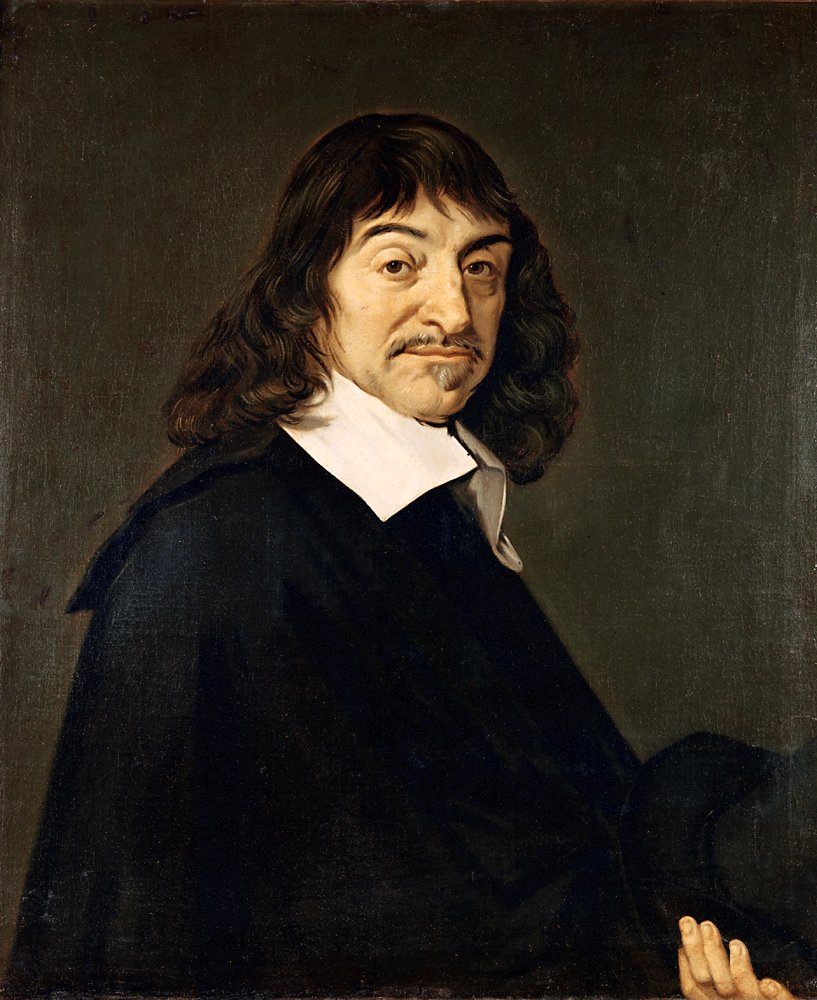
\includegraphics[scale=0.2]{img/Descartes.eps}
 \captionsetup{labelformat=empty}
 \caption{René Descartes (1596 - 1650). Portrait after Frans Hals, oil on canvas, Louvre Museum}
 \label{fig:Decartes}
\end{figure}
%\end{wrapfigure}

\index{Cartesian product} \index{Descartes}
Cartesian product, also known as direct product, is named after René Descartes, the great French philosopher, mathematician, and scientist. In the days of Descartes, Latin was a widely used academy language. He also had a Latinized name: Renatus Cartesius. Its adjective form is Cartesian. This is the reason why we say Cartesian product or Cartesian coordinate system today.

Descartes was born in La Haye, near Tours, France in 1596. His father was a member of the Parlement of Brittany at Rennes. His mother died a year after giving birth to him, and so he was not expected to survive. His father then remarried in 1600. Descartes lived with his grandmother at La Haye. His health was poor when he was a child. Throughout his childhood, up to his twenties, he was pale and had a persistent cough which was probably due to tuberculosis. It seems likely that he inherited these health problems from his mother.

In 1607, he entered the Jesuit college of La Flèche, where he was introduced to mathematics and physics, including Galileo's work. While in the school his health was poor and, instead of rising at 5 a.m. like the other boys, he was granted permission to remain in bed until 11 o'clock in the morning, a custom he maintained until the year of his death.

After graduation in 1614, he studied for two years at the University of Poitiers. He received a law degree in 1616 to comply with his father's wishes but he quickly decided that this was not the path he wanted to follow. He returned to Paris, then became a volunteer in the army of Maurice of Nassau. In the army, Descartes started studying mathematics and mechanics under the Dutch scientist Isaac Beeckman, and began to seek a unified science of nature.

After this time in Holland he left the service of Maurice of Nassau and travelled through Europe. In 1619 he joined the Bavarian army and was stationed in Ulm. An important event in his life was three dreams he had in November 1619. These he believed were sent by a divine spirit with the intention of revealing to him a new approach to philosophy. The ideas from these dreams would dominate much of his work from that time on.

From 1620 to 1628 Descartes travelled through Europe, spending time in Bohemia, Hungary, Germany, Holland, through Switzerland to Italy, then Venice and Rome. He returned Paris in 1625. His Paris home became a meeting place for philosophers and mathematicians and steadily became more and more busy. By 1628 Descartes, tired of the bustle of Paris, the house full of people, and of the life of travelling he had before, decided to settle down where he could work in solitude. He gave much thought to choosing a country suited to his nature and he chose Holland. What he longed for was somewhere peaceful where he could work away from the distractions of a city such as Paris yet still have access to the facilities of a city. It was a good decision which he did not seem to regret over the next twenty years. He told his friend Marin Mersenne\footnote{Mersenne was a French polymath, whose works touched a wide variety of fields. He is perhaps best known today among mathematicians for Mersenne prime numbers, in the form $M_n = 2^n − 1$ for some integer $n$. He had many contacts in the scientific world and has been called "the center of the world of science and mathematics during the first half of the 1600s".} where he was living so that he might keep in touch with the mathematical world, but otherwise he kept his place of residence a secret. Descartes wrote all his major work during his 20-plus years in the Netherlands, initiating a revolution in mathematics and philosophy. In 1633, Galileo was condemned by the Italian Inquisition, and Descartes abandoned plans to publish {\em Treatise on the World}, his work of the previous four years. Nevertheless, in 1637 he published parts of this work in three essays: {\em The Meteors}, {\em Dioptrics} and {\em Geometry}, preceded by an introduction, his famous {\em Discourse on the Method}.

In {\em Geometry}, Descartes exploited the discoveries he made with Pierre de Fermat. This later became known as Cartesian Geometry. Descartes continued to publish works concerning both mathematics and philosophy for the rest of his life. In 1641 he published a metaphysics treatise, {\em Meditations on First Philosophy}. It was followed in 1644 by {\em Principles of Philosophy}. He became the most influential philosophers in Europe.

In 1649 Queen Christina of Sweden persuaded Descartes to go to Stockholm. However the Queen wanted to draw tangents at 5 a.m. and Descartes broke the habit of his lifetime of getting up at 11 o'clock. After only a few months in the cold northern climate, walking to the palace for 5 o'clock every morning, he died of pneumonia February 1650 at the age of 54.

Descartes left the best known philosophical statement `` think, therefore I am'' (French: Je pense, donc je suis; Latin: cogito, ergo sum). Descartes laid the foundation for 17th-century continental rationalism. He was well-versed in mathematics as well as philosophy, and contributed greatly to science as well. He is credited as the father of analytical geometry, the bridge between algebra and geometry—used in the discovery of infinitesimal calculus and analysis. Descartes was also one of the key figures in the Scientific Revolution.

\vspace{5mm}

Symmetric to the Cartesian product of sets, there is a dual construct. From two sets $A$ and $B$, we can generate a disjoint union set (sum) $A + B$. For the element in the sum, in order to know which set $A$ or $B$ it comes from, we can add a tag:

\[
A + B = (A \times \{0\}) \cup (B \times \{1\})
\]

For every element $(x, tag)$ in $A + B$, if the $tag$ is 0, we know that $x$ comes from $A$, else if the $tag$ is 1, then $x$ comes from $B$. Hence the sum of finite set $\{1, 2, 3\}$ and $\{a, b\}$ is

\[
\{(1, 0), (2, 0), (3, 0), (a, 1), (b, 1)\}
\]

When programming, $A + B$ can be defined as:

\begin{mdframed}
\[
A + B = zip\ A\ \{0, ...\} \doubleplus zip\ B\ \{1, ...\}
\]
\end{mdframed}

If set $A$ and $B$ are the same algebraic structures, we can define the below objects and arrows:

\begin{center}
\begin{tikzpicture}
  \matrix (m) [matrix of math nodes,
               row sep=2em, column sep=2em, minimum width=2em]{
    a & A &        &       &        & B & b \\
      &   &        &       &        &   & \\
      &   & (a, 0) & A + B & (b, 1) &   & \\};
  \path[|->]
    (m-1-1) edge (m-3-3)
    (m-1-7) edge (m-3-5);
  \path[-stealth]
    (m-1-2) edge (m-3-4)
    (m-1-6) edge (m-3-4);
\end{tikzpicture}
\end{center}

\begin{wrapfigure}{R}{0.4\textwidth}
%\begin{figure}[htbp]
 \centering
 
\includegraphics[scale=0.06]{img/hands.eps}
 \captionsetup{labelformat=empty}
 \caption{}
 \label{fig:hands}
%\end{figure}
\end{wrapfigure}

The two constructions are symmetric. If rotate the two diagrams by 90 degree, laying $A$ on top of $B$, then the two problems appear left and right. They are symmetric like our two hands. We can find a lot of such symmetric concepts in category theory. Our world is full of symmetric things. When we understand one, we understand the dual one at the same time.

\subsection{Definition of product and coproduct}
\index{product} \index{coproduct}
\begin{definition}
For a pair of objects $A$ and $B$ in category $\pmb{C}$, a {\em wedge}

\[
\text{to} \quad \quad \quad \text{from}
\]

\index{wedge}
the pair $A, B$ is an object $X$ together with a pair of arrows

\begin{center}
\begin{tikzpicture}
  \matrix (m) [matrix of math nodes,
               row sep=2em, column sep=2em, minimum width=2em]{
      & A &  & A & \\
    X &   &  &   & X \\
      & B &  & B & \\};
  \path[-stealth]
    (m-2-1) edge (m-1-2)
    (m-2-1) edge (m-3-2)
    (m-1-4) edge (m-2-5)
    (m-3-4) edge (m-2-5);
\end{tikzpicture}
\end{center}

in the parent category $\pmb{C}$.
\end{definition}

For a given pair of objects $A, B$ in the category, there may be many wedges o one side or the other. We look for the `best possible' wedge, one that is as `near' the pair as possible. Technically, we look for a universal wedge. It leads to the below (pair of) definitions:

\begin{definition}
Given a pair object $A, B$ of a category $\pmb{C}$, a

\[
\text{product} \quad \quad \quad \text{coproduct}
\]

of the pair is a wedge:

\begin{center}
\begin{tikzpicture}
  \matrix (m) [matrix of math nodes,
               row sep=2em, column sep=2em, minimum width=2em]{
      & A &  & A & \\
    S &   &  &   & S \\
      & B &  & B & \\};
  \path[-stealth]
    (m-2-1) edge node [above] {$p_A$} (m-1-2)
    (m-2-1) edge node [below] {$p_B$} (m-3-2)
    (m-1-4) edge node [above] {$i_A$} (m-2-5)
    (m-3-4) edge node [below] {$i_B$} (m-2-5);
\end{tikzpicture}
\end{center}

with the following universal property. For each wedge

\begin{center}
\begin{tikzpicture}
  \matrix (m) [matrix of math nodes,
               row sep=2em, column sep=2em, minimum width=2em]{
      & A &  & A & \\
    X &   &  &   & X \\
      & B &  & B & \\};
  \path[-stealth]
    (m-2-1) edge node [above] {$f_A$} (m-1-2)
    (m-2-1) edge node [below] {$f_B$} (m-3-2)
    (m-1-4) edge node [above] {$f_A$} (m-2-5)
    (m-3-4) edge node [below] {$f_B$} (m-2-5);
\end{tikzpicture}
\end{center}

there is a unique arrow:

\[
 X \arrowto{m} S \quad \quad \quad S \arrowto{m} X
\]

such that,

\begin{center}
\begin{tikzpicture}
  \matrix (m) [matrix of math nodes,
               row sep=2em, column sep=2em, minimum width=2em]{
      & A &  & A & \\
    X & S &  & S & X \\
      & B &  & B & \\};
  \path[-stealth]
    % left
    (m-2-1) edge node [above] {$f_A$} (m-1-2)
    (m-2-1) edge node [below] {$f_B$} (m-3-2)
    (m-2-1) edge node [above] {$m$}   (m-2-2)
    (m-2-2) edge node [right] {$p_A$} (m-1-2)
    (m-2-2) edge node [right] {$p_B$} (m-3-2)
    % right
    (m-1-4) edge node [above] {$f_A$} (m-2-5)
    (m-3-4) edge node [below] {$f_B$} (m-2-5)
    (m-2-4) edge node [above] {$m$}   (m-2-5)
    (m-1-4) edge node [right] {$i_A$} (m-2-4)
    (m-3-4) edge node [right] {$i_B$} (m-2-4);
\end{tikzpicture}
\end{center}

\index{媒介箭头}
commutes. This arrow $m$ is the {\em mediating arrow} (or mediator) for the wedge on $X$.
\end{definition}

In this definition, the product or coproduct is not just an object $S$, but an object together with a pair of arrows. For any given $X$, the mediating arrow $m$ is unique. We say the diagram commutes, it means the arrows satisfy the following equations:

\[
\begin{array}{l}
f_A = p_A \circ m \\
f_B = p_B \circ m
\end{array}
\]

It immediately leads to this special case: If $X$ equals to $S$, then $m$ is an endo-arrow (points to itself).

\[
S \arrowto{m} S
\]

Hence $m$ must be identity arrow. The diagram then simplifies to:

\begin{center}
\begin{tikzpicture}
  \matrix (m) [matrix of math nodes,
               row sep=3em, column sep=3em, minimum width=2em]{
      & A &  & A & \\
    S & S &  & S & S \\
      & B &  & B & \\};
  \path[-stealth]
    % left
    (m-2-1) edge node [above] {$p_A$} (m-1-2)
    (m-2-1) edge node [below] {$p_B$} (m-3-2)
    (m-2-1) edge node [above] {$id_S$} (m-2-2)
    (m-2-2) edge node [right] {$p_A$} (m-1-2)
    (m-2-2) edge node [right] {$p_B$} (m-3-2)
    % right
    (m-1-4) edge node [above] {$i_A$} (m-2-5)
    (m-3-4) edge node [below] {$i_B$} (m-2-5)
    (m-2-4) edge node [above] {$id_S$} (m-2-5)
    (m-1-4) edge node [right] {$i_A$} (m-2-4)
    (m-3-4) edge node [right] {$i_B$} (m-2-4);
\end{tikzpicture}
\end{center}

Among the many wedges, the product and product are special, they are universal solutions. In other words, they are the `closest' or the `best' wedge. We can prove that product and coproduct are unique (see the appendix of this book). However, product and coproduct may not exist at the same time, it's also possible that neither does exist. Let's see what product and coproduct mean to set.

\begin{lemma}
Let $A$, $B$ be a pair of sets. Then the

\begin{center}
\begin{tabular}{ccc}
Cartesian product & \quad \quad \quad & disjoint union \\
$A \times B$ & \quad \quad \quad & $A + B$ \\
\end{tabular}
\end{center}

furnished with canonical functions form the

\begin{center}
product \quad \quad \quad coproduct
\end{center}

of the pair in the category $\pmb{Set}$.
\end{lemma}

The detailed proof can be found in the appendix of this book. In program environment, product is often realized with paired tuple $(a, b)$ and functions $fst, snd$. However, coproduct is sometimes realized with a dedicated data type.

\lstset{frame = single}
\begin{lstlisting}
data Either a b = Left a | Right b
\end{lstlisting}

The advantage is that we needn't the 0, 1 tags to mark if an element $x$ of type \texttt{Either a b} comes from \texttt{a} or \texttt{b}. The below example program handles the coproduct value through pattern matching:

\begin{lstlisting}
either :: (a -> c) -> (b -> c) -> Either a b -> c
either f _ (Left x)     =  f x
either _ g (Right y)    =  g y
\end{lstlisting}
\lstset{frame = none}

Let's see an example, consider the coproduct \texttt{Either String Int}. It is either a string, like \texttt{s = Left "hello"}; or an integer, like \texttt{n = Right 8}. If it is a string, we want to count its length; if it is a number, we want to double it. To do this, we can utilize the $either$ function: \texttt{either length (*2) x}.

Thus \texttt{either length (*2) s} will count the length of string ``hello'' which gives 5; while \texttt{either length (*2) n} will double 8 to give 16. Some programming environments have the concept of \texttt{union} or \texttt{enum} data type to realize coproduct partially. In the future, we sometimes call the two arrows of the coproduct $left$ and $right$ respectively.

\subsection{The properties of product and coproduct}

According to the definition of product and coproduct, for any wedge consist of $X$ and arrows, the mediator arrow $m$ is uniquely determined. In category $\pmb{Set}$, the mediator arrow can be defined as the following:

\[
\begin{array}{ccc}
\text{product} & & \text{coproduct} \\
m(x) = (a, b) & \quad \quad &
\begin{cases}
m (a, 0) = p(a) \\
m (b, 1) = q(b)
\end{cases}
\end{array}
\]

For a generic category, how to define the mediator arrow? To do that, we introduce two dedicated symbols for arrow operation. Given any wedge:

\begin{center}
\begin{tikzpicture}
  \matrix (m) [matrix of math nodes,
               row sep=2em, column sep=2em, minimum width=2em]{
      & A &  & A & \\
    X &   &  &   & X \\
      & B &  & B & \\};
  \path[-stealth]
    (m-2-1) edge node [above] {$f$} (m-1-2)
    (m-2-1) edge node [below] {$g$} (m-3-2)
    (m-1-4) edge node [above] {$f$} (m-2-5)
    (m-3-4) edge node [below] {$g$} (m-2-5);
\end{tikzpicture}
\end{center}

Define

\[
m = \langle f, g \rangle \quad \quad \quad m =[f, g]
\]

which satisfy:

\[
\begin{array}{rcl}
\begin{cases}
fst \circ m = f \\
snd \circ m = g
\end{cases}
& \quad \quad &
\begin{cases}
m \circ left = f \\
m \circ right = g
\end{cases}
\end{array}
\]

Hence the following diagram commutes:

\begin{center}
\begin{tikzpicture}
  \matrix (m) [matrix of math nodes,
               row sep=3em, column sep=3em, minimum width=2em]{
      & A &  & A & \\
    X & A \times B &  & A + B & X \\
      & B &  & B & \\};
  \path[-stealth]
    % left
    (m-2-1) edge node [above] {$f$} (m-1-2)
    (m-2-1) edge node [below] {$g$} (m-3-2)
    (m-2-1) edge node [above] {$\langle f, g \rangle$}   (m-2-2)
    (m-2-2) edge node [right] {$fst$} (m-1-2)
    (m-2-2) edge node [right] {$snd$} (m-3-2)
    % right
    (m-1-4) edge node [above] {$f$} (m-2-5)
    (m-3-4) edge node [below] {$g$} (m-2-5)
    (m-2-4) edge node [above] {$[f, g]$}   (m-2-5)
    (m-1-4) edge node [left] {$left$} (m-2-4)
    (m-3-4) edge node [left] {$right$} (m-2-4);
\end{tikzpicture}
\end{center}

\index{Cancellation law}
From this pair of diagrams, we can obtain some important properties for product and coproduct directly. First is the {\em cancellation law}:

\[
\begin{array}{rcl}
\begin{cases}
fst \circ \langle f, g \rangle = f \\
snd \circ \langle f, g \rangle = g
\end{cases}
& \quad \quad &
\begin{cases}
[f, g] \circ left = f \\
[f, g] \circ right = f
\end{cases}
\end{array}
\]

\index{reflection law}
For product, if arrow $f$ equals to $fst$, and arrow $g$ equals to $snd$, then we obtain the special case of identity arrow mentioned in previous section. Similarly for the coproduct, if arrow $f$ equals to $left$, and arrow $g$ equals to $right$, then the mediator arrow is also the identity arrow. We call this property the {\em reflection law}:

\[
id = \langle fst, snd \rangle \quad \quad \quad id = [left, right]
\]

If there exists another wedge $Y$ and arrows $h$ and $g$, together with $f, g$ they satisfy the following conditions:

\[
\begin{array}{ccc}
  \text{product} & & \text{coproduct} \\
  \begin{cases}
  h \circ \phi = f \\
  k \circ \phi = g
  \end{cases}
  & \quad \quad &
  \begin{cases}
  \phi \circ h = f \\
  \phi \circ k = g
  \end{cases}
\end{array}
\]

For

\[
\langle h, k \rangle \circ \phi \quad \quad \quad \phi \circ [h, k]
\]

\index{fusion law}
Substitute $m$, and apply cancellation law, then we obtain the {\em fusion law}:

\[
\begin{array}{ccc}
  \text{product} & & \text{coproduct} \\
  \begin{cases}
  h \circ \phi = f \\
  k \circ \phi = g
  \end{cases} \Rightarrow
    \langle h, k \rangle \circ \phi = \langle f, g \rangle
  & \quad \quad &
  \begin{cases}
  \phi \circ h = f \\
  \phi \circ k = g
  \end{cases} \Rightarrow
    \phi \circ [h, k] = [f, g]
\end{array}
\]

It means:

\[
\langle h, k \rangle \circ \phi = \langle h \circ \phi, k \circ \phi \rangle
\quad \quad \quad
\phi \circ [h, k] = [\phi \circ h, \phi \circ k]
\]

We'll see later, these laws play important roles during algorithm reasoning, simplification, and optimization.

\subsection{Functors from products and coproducts}
\index{bifunctor} \index{binary functor}
With product in category theory, we can introduce the concept of {\em bifunctor} (also known as binary functor). The functors we've seen so far transform the objects from one category to the objects in another category; and also transforms arrows from one category to the other. The bifunctor applies to the product of two categories $\pmb{C}$ and $\pmb{D}$. In other words, the source is $\pmb{C} \times \pmb{D}$. Bifunctor transforms objects as the following:

\[
\begin{array}{rcl}
\pmb{C} \times \pmb{D} & \longrightarrow & \pmb{E} \\
A \times B & \longmapsto & \mathbf{F}(A \times B) \\
\end{array}
\]

Besides objects, functor must transform arrows as well. For the arrow $f$ in category $\pmb{C}$, and the arrow $g$ in category $\pmb{D}$, what the bifunctor behaves? Observe the below diagram:

\begin{center}
\begin{tikzpicture}
  \matrix (m) [matrix of math nodes,
               row sep=2.5em, column sep=2.5em, minimum width=2em]{
     A & & \mathbf{F}(A \times B) \\
     C & \mathbf{F}(C \times D) & \\
       & D & B \\};
  \path[-stealth]
    (m-1-1) edge (m-1-3)
    (m-2-1) edge (m-2-2)
    (m-1-1) edge node [left] {$f$} (m-2-1)
    (m-1-3) edge node [above] {$\mathbf{F}(f \times g)$} (m-2-2)
    (m-3-2) edge (m-2-2)
    (m-3-3) edge (m-1-3)
    (m-3-3) edge node [below] {$g$} (m-3-2);
  \draw
    (-2.5, 0.5) circle[x radius=2em, y radius=4em] % C
    (0.5, -1.5) circle[x radius=5em, y radius=2em] % D
    (0.5, 0.5) circle[x radius=5.5em, y radius=3.5em]; % E
  \path
    (-2.5, -1.5) node {$\pmb{C}$}
    (1.5, -2.5) node {$\pmb{D}$}
    (3, 0.5) node {$\pmb{E}$};
\end{tikzpicture}
\end{center}

From this diagram, the arrow $A \arrowto{f} C$ and $B \arrowto{g} D$ are sent to the new arrow in category $\pmb{E}$ through the functor $\mathbf{F}$. The source object is $\mathbf{F}(A \times B)$, and the target object is $\mathbf{F}(C \times D)$. To do that, we first define the product of two arrows $f$ and $g$, it applies to the product of $A$ and $B$. For every $(a, b) \in A \times B$, it behaves as below:

\[
(f \times g)(a, b) = (f\ a\ , g\ b)
\]

The bifunctor $F$ applies to this product of arrows $f \times g$, sends it to the new arrow 头$\mathbf{F}(f \times g)$. Hence the final definition for bifunctor is as below:

\[
\begin{array}{rcl}
\pmb{C} \times \pmb{D} & \longrightarrow & \pmb{E} \\
A \times B & \longmapsto & \mathbf{F}(A \times B) \\
f \times g & \longmapsto & \mathbf{F}(f \times g) \\
\end{array}
\]

\begin{mdframed}
We need verify the bifunctor satisfies the two conditions as a functor: the identity condition and the composition condition. \textbf{Readers can skip the proof in this box}.

\[
\begin{array}{l}
\mathbf{F}(id \times id) = id \\
\mathbf{F}((f \circ f') \times (g \circ g')) = \mathbf{F}(f \times g) \circ \mathbf{F} (f' \times g')
\end{array}
\]

\begin{proof}
We treat the product as an object. If we prove the following two conditions essentially, then the proof for the bifunctor can be deduced from it through the known result of normal functors.

\[
\begin{array}{l}
id \times id = id \\
(f \circ f') \times (g \circ g') = (f \times g) \circ (f' \times g')
\end{array}
\]

We start from proving the identity condition. For all $(a, b) \in A \times B$, we have:

\[
\begin{array}{rcll}
(id \times id)(a, b) & = & (id(a), id(b)) & \text{product of arrows} \\
                     & = & (a, b) & \text{definition of $id$} \\
                     & = & id(a, b) & \text{reverse of $id$} \\
\end{array}
\]

Next we prove the composition condition.

\[
\begin{array}{rcll}
((f \circ f') \times (g \circ g'))(a, b) & = & ((f \circ f')\ a, (g \circ g')\ b) & \text{product of arrows} \\
    & = & (f(f'(a)), g(g'(b))) & \text{arrow composition} \\
    & = & (f \times g)(f'(a), g'(b)) & \text{reverse of arrows product} \\
    & = & (f \times g)((f' \times g')(a, b)) & \text{reverse of arrows product} \\
    & = & ((f \times g) \circ (f' \times g'))(a, b)
\end{array}
\]

Hence proved the bifunctor satisfies both functor conditions.
\end{proof}
\end{mdframed}

Similar to $fmap$, some programming environments have limitation to use the same symbol for both object and arrow mapping. To solve that, we can define a dedicated $bimap$ for bifunctor arrow mapping. We need every bifunctor $\mathbf{F}$ satisfy:

\[
bimap : (A \to C) \to (B \to D) \to (\mathbf{F}\ A \times B \to \mathbf{F}\ C \times D)
\]

It means, if $\mathbf{F}$ is a bifunctor, then it send the two arrows $A \arrowto{g} C$ and $B \arrowto{h} D$ to an arrow that maps from $\mathbf{F}\ A \times B$ to $\mathbf{F}\ C \times D$.

With the concept of bifunctor, we can define product and coproduct functors. We'll use the infix notation. Denote:

\begin{center}
\begin{tabular}{ccc}
 product functor as & \quad \quad \quad & coproduct functor as \\
 $\times$  & \quad \quad \quad & $+$ \\
\end{tabular}
\end{center}

Given two objects, the product functor maps them to their product; while the coproduct functor maps them to their coproduct. For arrows, define:

\[
f \times g = \langle f \circ fst, g \circ snd \rangle
\quad \quad \quad
f + g = [left \circ f, right \circ g]
\]

\begin{mdframed}
We need verify the two functor conditions, \textbf{Readers can skip the proof in this box}. For the identity condition. Substitute $f, g$ with $id$:

\[
\begin{array}{lr}
  \begin{array}{cll}
    & id \times id & \\
  = & \langle id \circ fst, id \circ snd \rangle & \text{Definition of $\times$} \\
  = & \langle fst, snd \rangle & \text{Definition of $id$} \\
  = & id & \text{Reflection law} \\
  \end{array}
  &
  \begin{array}{cll}
    & id + id & \\
  = & [ left \circ id, right \circ id ] & \text{Definition of $+$} \\
  = & [ left, right] & \text{Definition of $id$} \\
  = & id & \text{Reflection law} \\
  \end{array}
\end{array}
\]

Next we need verify the composition condition:

\[
\begin{array}{ccc}
\text{product} & \quad \quad & \text{coproduct} \\
 (f \times g) \circ (f' \times g') = f \circ f' \times g \circ g'
 & \quad \quad &
 (f + g) \circ (f' + g') = f \circ f' + g \circ g'
\end{array}
\]

\index{absorption law}
In order to prove it, we will first prove the {\em absorption law} for

\[
\begin{array}{ccc}
  \text{product} & \quad \quad & \text{coproduct} \\
  (f \times g) \circ \langle p, q \rangle = \langle f \circ p, g \circ q \rangle
  & \quad \quad &
  [p, q] \circ (f + g) = [p \circ f, q \circ g]
\end{array}
\]

We only give the proof for the product on the left. the coproduct side can be proved similarly. We leave it as the exercise.

\[
\begin{array}{cll}
   & (f \times g) \circ \langle p, q \rangle & \\
 = & \langle f \circ fst, g \circ snd \rangle \circ \langle p, q \rangle & \text{Definition of $\times$} \\
 = & \langle f \circ fst \circ \langle p, q \rangle, g \circ snd \circ \langle p, q \rangle \rangle & \text{Fusion law} \\
 = & \langle f \circ p, g \circ q \rangle & \text{Cancellation law} \\
\end{array}
\]

Using the absorption law, let $p = f' \circ fst, q = g' \circ snd$, we can verify the composition condition:

\[
\begin{array}{cll}
  & (f \times g) \circ (f' \times g') & \\
= & (f \times g) \circ \langle f' \circ fst, g' \circ snd \rangle & \text{Definition of $\times$ for the 2nd term} \\
= & (f \times g) \circ \langle p, q \rangle & \text{Substitute with $p, q$} \\
= & \langle f \circ p, g \circ q \rangle & \text{absorption law} \\
= & \langle f \circ f' \circ fst, g \circ g' \circ snd \rangle & \text{Substitute back $p, q$} \\
= & \langle (f \circ f') \circ fst, (g \circ g') \circ snd \rangle & \text{association law} \\
= & (f \circ f') \times (g \circ g') & \text{Reverse of $\times$} \\
\end{array}
\]

\end{mdframed}

\index{bimap}
Product functor is an instance of bifunctor. We can define it as $bimap$ like below:

\[
\begin{array}{l}
bimap : (A \to C) \to (B \to D) \to (A \times B \to C \times D) \\
bimap\ f\ g\ (x, y) = (f\ x,\ g\ y)
\end{array}
\]

With the \texttt{Either} type to realize the coproduct functor, the corresponding $bimap$ can be defined like this:

\[
\begin{array}{l}
bimap : (A \to C) \to (B \to D) \to (Either\ A\ B \to Either\ C\ D) \\
bimap\ f\ g\ (left\ x) = left\ (f\ x) \\
bimap\ f\ g\ (right\ y) = right\ (g\ y)
\end{array}
\]

\begin{Exercise}
\Question{For any two objects in a poset, what is their product? what is their coproduct?}
%\Question{考虑集合范畴$\pmb{Set}$,积中的两个箭头$fst, snd$是右消去(epic)的么?余积中的两个箭头$left, right$是左消去(monic)的么?}
\Question{Prove the absorption law for coproduct, and verify the coproduct functor satisfies composition condition.}
\end{Exercise}

\section{Natural transformation}

Saunders Mac Lane, one of the founders of category theory, is said to have remarked, "I didn't invent categories to study functors; I invented them to study natural transformations."

艾伦伯格和麦克兰恩在1940年代发展范畴论时,他们想解释为何某些构造是“自然”的,而某些不是。现在这一术语被命名为“自然变换”。麦克兰恩曾说:“我并非为了研究函子而发明了范畴,我发明它们是为了研究自然变换。”通过前面介绍的范畴和函子,我们可以说在范畴论中,箭头用于比较对象,而函子用于比较范畴。那么我们用什么比较函子呢?自然变换正是用于比较函子的工具。

考虑下面的两个函子:

\begin{center}
\begin{tikzpicture}
  \matrix (m) [matrix of math nodes,
               row sep=3em, column sep=4em, minimum width=2em]{
     \pmb{Src} & \pmb{Trg} \\};
  \path[-stealth]
    (m-1-1.north east) edge node [above] {$\mathbf{F}$} (m-1-2.north west)
    (m-1-1.south east) edge node [below] {$\mathbf{G}$} (m-1-2.south west);
\end{tikzpicture}
\end{center}

它们联系两个同样的范畴,或者都是协变的,或者都是反变的。我们怎样比较它们呢?由于函子既映射对象,又映射箭头,所以我们也得既比较函子映射后的对象,也比较函子映射后的箭头。考虑$\pmb{Src}$中的任意对象$A$,它被两个函子映射成$\pmb{Trg}$中的两个对象$\mathbf{F}A$和$\mathbf{G}A$。我们要研究的是从$\mathbf{F}A$到$\mathbf{G}A$之间的箭头

\[
\mathbf{F}A \arrowto{\phi_A} \mathbf{G}A
\]

并且除了$A$外,我们对$\pmb{Src}$中的所有对象做同样的研究。

\index{自然变换}
\begin{definition}
任给如上图所示的一对函子$\mathbf{F}, \mathbf{G}$,一个自然变换

\[
F \arrowto{\phi} G
\]

是由$A$索引的在$\pmb{Trg}$中的一族箭头

\[
\mathbf{F}A \arrowto{\phi_A} \mathbf{G}A
\]

并且对$\pmb{Src}$中的任意箭头$A \arrowto{f} B$,下面的方形都是可交换的。

\begin{center}
\begin{tikzpicture}
  \matrix (m) [matrix of math nodes,
               row sep=3em, column sep=3em, minimum width=2em]{
     \mathbf{F}A & \mathbf{G}A & A & \mathbf{F}A & \mathbf{G}A \\
     \mathbf{F}B & \mathbf{G}B & B & \mathbf{F}B & \mathbf{G}B \\};
  \path[-stealth]
    % left covariant
    (m-1-1) edge node [above] {$\phi_A$} (m-1-2)
    (m-2-1) edge node [below] {$\phi_B$} (m-2-2)
    (m-1-1) edge node [left] {$\mathbf{F}(f)$} (m-2-1)
    (m-1-2) edge node [right] {$\mathbf{G}(f)$} (m-2-2)
    % middle
    (m-1-3) edge node [left] {$f$} (m-2-3)
    % right contravariant
    (m-1-4) edge node [above] {$\phi_A$} (m-1-5)
    (m-2-4) edge node [below] {$\phi_B$} (m-2-5)
    (m-2-4) edge node [left] {$\mathbf{F}(f)$} (m-1-4)
    (m-2-5) edge node [right] {$\mathbf{G}(f)$} (m-1-5);
\end{tikzpicture}

\text{协变} \quad \quad \quad \text{反变}
\end{center}
\end{definition}

从自然变换的范畴图中,我们看到任何一个箭头$f$,都对应一个可交换的方形。对于协变的情况,可交换意味着对于任何箭头$f$,下面的关系成立:

\[
\mathbf{G}(f) \circ \phi_A= \phi_B \circ \mathbf{F}(f)
\]

\subsection{自然变换的例子}

自然变换是在范畴、箭头、函子之上的又一层抽象。我们举一些具体的例子来帮助理解这一重要的概念。

\begin{example}
第一个例子是前缀枚举函数$inits$。任给一个字符串或者列表,$inits$可以枚举出所有的前缀,例如:

\lstset{frame=none}
\begin{lstlisting}
inits "Mississippi" = ["","M","Mi","Mis","Miss","Missi","Missis",
        "Mississ","Mississi","Mississip","Mississipp","Mississippi"]

inits [1, 2, 3, 4] = [[],[1],[1,2],[1,2,3],[1,2,3,4]]
\end{lstlisting}

概括来说,$inits$的行为如下:

\[
inits [a_1, a_2, ..., a_n] = [[], [a_1], [a_1, a_2], ..., [a_1, a_2, ..., a_n]]
\]

考虑集合范畴$\pmb{Set}$,对于任何对象,也就是集合$A$(或者说是类型$A$),都存在被$A$索引的$inits$箭头:

\[
inits_A : \mathbf{List} A \to \mathbf{List}(\mathbf{List} A)
\]

其中一个函子是列表函子$\mathbf{List}$,另一个函子是嵌套列表函子$\mathbf{List}\ \mathbf{List}$。

如果我们用“[]”简记法,这个箭头也可以表示为:

\[
[A] \arrowto{inits_A} [[A]]
\]

我们接下来要验证,对任何函数$A \arrowto{f} B$,有:

\[
\mathbf{List}(\mathbf{List}(f)) \circ inits_A = inits_B \circ \mathbf{List}(f)
\]

也就是说,要验证如下的方形范畴图是可交换的。

\begin{center}
\begin{tikzpicture}
  \matrix (m) [matrix of math nodes,
               row sep=3em, column sep=3em, minimum width=2em]{
     A & \lbrack A \rbrack & \lbrack \lbrack A \rbrack \rbrack \\
     B & \lbrack B \rbrack & \lbrack \lbrack B \rbrack \rbrack \\};
  \path[-stealth]
    (m-1-1) edge node [left] {$f$} (m-2-1)
    % square
    (m-1-2) edge node [above] {$init_A$} (m-1-3)
    (m-2-2) edge node [below] {$init_B$} (m-2-3)
    (m-1-2) edge node [left] {$\mathbf{List}(f)$} (m-2-2)
    (m-1-3) edge node [right] {$\mathbf{List}(\mathbf{List}(f))$} (m-2-3);
\end{tikzpicture}
\end{center}

\begin{proof}
我们利用前面小节中针对列表函子定义的$fmap$来证明可交换性。对任意$A$中的$n$个元素$a_1, a_2, ..., a_n$,令$B$中的$n$个元素$b_1, b_2, ..., b_n$满足:$f(a_1) = b_1, f(a_2) = b_2, ..., f(a_n) = b_n$。我们有:

\[
\begin{array}{cll}
  & \mathbf{List}(\mathbf{List}(f)) \circ init_A [a_1, ..., a_n] & \\
= & fmap_{[[]]}(f) \circ init_A [a_1, ..., a_n] & \text{使用$fmap$} \\
= & fmap_{[[]]}(f) [[], [a_1], ..., [a_1, a_2, ..., a_n]] & \text{$inits$的定义} \\
= & map(map\ f) [[], [a_1], ..., [a_1, a_2, ..., a_n]] & \text{列表函子的$fmap$等价于$map$} \\
= & [map\ f\ [], map\ f\ [a_1], ..., map\ f\ [a_1, a_2, ..., a_n]] & \text{$map$的定义} \\
= & [[], [f(a_1)], ..., [f(a_1), f(a_2), ..., f(a_n)]] & \text{对每个子列表应用$map\ f$} \\
= & [[], [b_1], ..., [b_1, b_2, ..., b_n]] & \text{$f$的定义} \\
= & init_B\ [b_1, b_2, ..., b_n] & \text{反向用$init$的定义} \\
= & init_B\ [f(a_1), f(a_2), ..., f(a_n)] & \text{反向用$f$的定义} \\
= & init_B \circ map(f)\ [a_1, a_2, ..., a_n] & \text{反向用$map\ f$} \\
= & init_B \circ fmap_{[]}(f) [a_1, ..., a_n] & \text{列表函子的$fmap$等价于$map$} \\
= & init_B \circ \mathbf{List}(f) [a_1, ..., a_n] & \\
\end{array}
\]
\end{proof}

所以$inits : \mathbf{List} \to \mathbf{List} \circ \mathbf{List}$的确是一个自然变换。
\end{example}

\begin{example}
我们举的第二个例子叫做$safeHead$,它的行为是安全地获取列表中的第一个元素。所谓“安全”,就是说它能够处理空列表Nil的情况。为此我们可以使用前面介绍过的可能函子$\mathbf{Maybe}$。它的定义如下:

\[
\begin{array}{l}
safeHead : [A] \to \mathbf{Maybe}\ A \\
safeHead\ [] = Nothing \\
safeHead\ (x:xs) = Just\ x
\end{array}
\]

同样在集合范畴,任何类型$A$是一个对象,它索引的箭头$safeHead$为:

\[
[A] \arrowto{safeHead_A} \mathbf{Maybe}\ A
\]

这里的两个函子分别是列表函子和可能函子。我们接下来要验证,对于任何箭头(函数)$A \arrowto{f} B$,下面的方形范畴图是可交换的:

\begin{center}
\begin{tikzpicture}
  \matrix (m) [matrix of math nodes,
               row sep=3em, column sep=5em, minimum width=2em]{
     A & \lbrack A \rbrack & \mathbf{Maybe}\ A \\
     B & \lbrack B \rbrack & \mathbf{Maybe}\ B \\};
  \path[-stealth]
    (m-1-1) edge node [left] {$f$} (m-2-1)
    % square
    (m-1-2) edge node [above] {$safeHead_A$} (m-1-3)
    (m-2-2) edge node [below] {$safeHead_B$} (m-2-3)
    (m-1-2) edge node [left] {$\mathbf{List}(f)$} (m-2-2)
    (m-1-3) edge node [right] {$\mathbf{Maybe}(f)$} (m-2-3);
\end{tikzpicture}
\end{center}

也就是要证明:

\[
  \mathbf{Maybe}(f) \circ safeHead_A = safeHead_B \circ \mathbf{List}(f)
\]

\begin{proof}
我们分两种情况证明。第一种情况是空列表:

\[
\begin{array}{cll}
  & \mathbf{Maybe}(f) \circ safeHead_A\ [] & \\
= & \mathbf{Maybe}(f)\ Nothing & \text{$safeHead$的定义} \\
= & Nothing & \text{$fmap\ f\ Nothing$的定义} \\
= & safeHead_B\ [] & \text{反向用$safeHead$的定义} \\
= & safeHead_B \circ \mathbf{List}(f)\ [] & \text{反向用$fmap\ f\ []$的定义} \\
\end{array}
\]

第二种情况是非空列表$(x:xs)$:

\[
\begin{array}{cll}
  & \mathbf{Maybe}(f) \circ safeHead_A\ (x:xs) & \\
= & \mathbf{Maybe}(f)\ (Just\ x) & \text{$safeHead$的定义} \\
= & Just\ f(x) & \text{$fmap\ f\ Just\ x$的定义} \\
= & safeHead_B\ (f(x) : fmap\ f\ xs) & \text{反向用$safeHead$的定义} \\
= & safeHead_B \circ \mathbf{List}(f)\ (x:xs) & \text{反向用$fmap\ f\ (x:xs)$的定义} \\
\end{array}
\]

综合这两种情况,就证明了$safeHead : \mathbf{List} \to \mathbf{Maybe}$的确是自然变换。
\end{proof}
\end{example}

我们总结一下这两个自然变换的例子。从范畴中的任意对象$A$开始(对于集合范畴,相当于一个集合$A$;对于编程,相当于一个类型$A$),通过一个函子$\mathbf{F}$,将其映射为对象$\mathbf{F}A$(对于集合范畴,$\mathbf{F}A$是另一个集合;对于编程,$\mathbf{F}A$是另一个类型),而另一函子$\mathbf{G}$将以映射为$\mathbf{G}A$。自然变换$\phi$经由$A$索引的箭头(在集合范畴中是一个映射;在编程中是一个函数)\footnote{也称在$A$上的部分(The component at $A$)},形如:

\[
\phi_A : \mathbf{F} A \to \mathbf{G} A
\]

现在,我们说不仅对$A$,而是对\textbf{所有}对象进行抽象,这样就得到了一族箭头(在编程中,就是一个\textbf{多态函数}\footnote{我们可以联想到面向对象编程中的多态函数和泛型编程中的模板函数。}):

\[
\phi : \forall A \cdot \mathbf{F} A \to \mathbf{G} A
\]

例如在Haskell中,可以这样写\footnote{Haskell中有一个ExplicitForAll的选项,我们在下一章介绍构造——叠加融合律(build/fold fusion law)时会再次遇到它。}:

\lstset{frame=single}
\begin{lstlisting}
phi :: forall a . F a -> G a
\end{lstlisting}

通常我们不需要明确标明\texttt{forall a},这样自然变换就可以写为:

\begin{lstlisting}
phi : F a -> G a
\end{lstlisting}

回顾此前的两个例子,我们可以知道$inits$和$safeHead$的类型分别为:

\begin{lstlisting}
inits :: [a] -> [[a]]

safeHead :: [a] -> Maybe a
\end{lstlisting}

它们仅仅是把\texttt{phi}换成了各自的名字,把$F, G$换成了各自的函子。

\subsection{自然同构}

我们说自然变换是用来比较函子的。仿照抽象代数中同构的含义,我们需要定义什么情况下认为两个函子是“等价”的。

% natural isomorphism
\index{自然同构}
\begin{definition}
我们称两个函子$\mathbf{F}$和$\mathbf{G}$间的\textbf{自然同构}是一个自然变换:

\[
  \mathbf{F} \arrowto{\phi} \mathbf{G}
\]

使得对每个源范畴中的对象$A$,被索引的箭头

\[
  \mathbf{F}A \arrowto{\phi_A} \mathbf{G}A
\]

都是目的范畴中的同构。
\end{definition}

有时我们也说自然同构的两个函子是自然等价的。 % naturally equivalent

我们举一个极端的例子$swap$。对于任意两个对象的积$A \times B$,$swap$将其对换为$B \times A$:

\[
\begin{array}{l}
swap : A \times B \to B \times A \\
swap\ (a, b) = (b, a)
\end{array}
\]

$swap$是一个自然变换,它作用于两个二元函子,恰巧这两个二元函子都是积函子,即:$\mathbf{F} = \mathbf{G} = \times$

由于是二元函子,所以对任意两个箭头$A \arrowto{f} C$和$B \arrowto{g} D$,我们需要下面的自然条件使得范畴图可交换:

% natural condition

\[
(g \times f) \circ swap_{A \times B} = swap_{C \times D} \circ (f \times g)
\]

\begin{center}
\begin{tikzpicture}
  \matrix (m) [matrix of math nodes,
               row sep=3em, column sep=5em, minimum width=2em]{
       & B          & D \\
     A & A \times B & B \times A \\
     C & C \times D & D \times C \\};
  \path[-stealth]
    (m-2-1) edge node [left] {$f$} (m-3-1)
    (m-1-2) edge node [above] {$g$} (m-1-3)
    % square
    (m-2-2) edge node [above] {$swap_{A \times B}$} (m-2-3)
    (m-3-2) edge node [below] {$swap_{C \times D}$} (m-3-3)
    (m-2-2) edge node [left] {$f \times g$} (m-3-2)
    (m-2-3) edge node [right] {$g \times f$} (m-3-3);
\end{tikzpicture}
\end{center}

证明这一点很简单,只要任选两个对象的积$(a, b)$和$(c, d)$分别代入自然条件的左右两侧即可。我们把它留给读者作为练习。

虽然两个函子都是积函子,我们还是来证明一下它们是自然同构的。对于任何两个对象的积$A \times B$,注意到:

\[
swap_{A \times B} \circ swap_{B \times A} = id
\]

也就是说$swap$是一个一一映射,因此它在目标范畴中是同构的。这样就证明了自然同构。

以上的三个例子$inits, safeHead, swap$都是多态函数,它们也都是自然变换。这不是一个巧合。在函数式编程中,所有的多态函数都是自然映射\cite{Wadler-1989}。

\begin{Exercise}
\Question{证明$swap$满足自然变换的条件$(g \times f) \circ swap = swap \circ (f \times g)$}
\Question{证明多态函数$length$是一个自然变换,其定义如下:
\[
\begin{array}{l}
length : [A] \to Int \\
length\ [] = 0 \\
length\ (x:xs) = 1 + length\ xs
\end{array}
\]
}
\Question{自然变换也可以进行组合,考虑两个自然变换$\mathbf{F} \arrowto{\phi} \mathbf{G}$}和$\mathbf{G} \arrowto{\psi} \mathbf{H}$,对于任意箭头$A \arrowto{f} B$,试画出自然变换组合$\phi \circ \psi$的范畴图,并列出可交换性的条件。
\end{Exercise}

\section{数据类型}

我们已经简单介绍了范畴论中的最基本概念,包括范畴、函子、自然变换。接下来我们了解一下如何通过这些基本组件实现较复杂的数据类型。

\subsection{起始对象和终止对象}
让我们先认识两个最简单的数据类型,起始对象(initial object)和终止对象(terminal object或final object)。这两个对象也像左右手一样是对偶的,它们虽然简单,可是并不容易理解。

\index{起始对象} \index{终止对象}
\begin{definition}
在任意范畴$\pmb{C}$中,如果有一个特殊的对象$S$,使得范畴中的每个对象$A$都有一个唯一的箭头

\[
  S \longrightarrow A \quad \quad \quad A \longrightarrow S
\]

也就是说$S$存在

\begin{center}
  指向所有其它对象  \quad \quad \quad 从所有其它对象指向自己
\end{center}
的唯一箭头,我们称这个对象$S$为

\begin{center}
  起始对象 \quad \quad \quad 终止对象
\end{center}
\end{definition}

习惯上,我们用0表示起始对象,1表示终止对象。所以对任何对象$A$有:

\[
  0 \longrightarrow A \quad \quad \quad A \longrightarrow 1
\]

为什么说起始对象和终止对象是对偶的呢?如果$S$是范畴$\pmb{C}$中的起始对象,我们只要把所有的箭头都反向,则$S$就成了范畴$\pmb{C}^{op}$中的终止对象。一个范畴可能没有起始对象或终止对象,或者两个都没有,但如果有的话,起始对象或者终止对象在同构的意义下是唯一的。

我们只证明起始对象的同构唯一性,终止对象可以通过对偶性得到证明。

\begin{proof}
假设除0外还存在另一个起始对象0'。考虑起始对象0,根据定义一定存在从0指向0'的箭头$f$;反过来,当考虑起始对象0'的时候,也一定存在从0'指向0的箭头$g$。但是根据范畴公理,一定也有从0指向自己的箭头$id_0$和从0'指向自己的箭头$id_0'$。根据起始对象定义中箭头的唯一性,一定有:

\[
  id_0 = f \circ g \quad \text{和} \quad id_{0'} = g \circ f
\]

这一关系可从下面的范畴图看出。

\begin{center}
\begin{tikzpicture}
  \matrix (m) [matrix of math nodes,
               row sep=3em, column sep=4em, minimum width=2em]{
     0 & 0' \\};
  \path[-stealth]
    (m-1-1.north east) edge node [above] {$f$} (m-1-2.north west)
    (m-1-2.south west) edge node [below] {$g$} (m-1-1.south east);
  \draw[->]
    (m-1-1.north west) arc[radius=5mm, start angle=45, end angle=315] node [pos=0.5, left] {$id_0$}; % (m-1-1.south west)
  \draw[->]
    (m-1-2.south east) arc[radius=5mm, start angle=-135, end angle=135] node [pos=0.5, right] {$id_{0'}$}; % (m-1-2.north east);
\end{tikzpicture}
\end{center}

这就证明了0和0'是同构的。换言之,在同构的意义下,起始对象是唯一的。
\end{proof}

\index{零对象}
特别地,如果一个对象既是起始对象,又是终止对象,我们称之为零对象(zero object或null object)。一个范畴并不一定有零对象。

接下来我们通过一些例子,由简到难说明起始对象和终止对象对应着什么样的数据类型。

\begin{example}
考虑一个偏序集,箭头为序关系。如果一个偏序集存在最小值,则这个最小值就是起始对象;类似地,如果存在最大值,则最大值就是终止对象。例如《红楼梦》人物的有限集合\{贾宝玉、贾政、贾代善、贾源\}中,序关系为祖先关系。这样贾宝玉就是起始对象,贾源就是终止对象。而斐波那契数列组成的集合\{1, 1, 2, 3, 5, 8, ...\},序关系为小于等于。1是最小值,是起始对象;但是没有终止对象。注意斐波那契数列中有两个1,但是它们在小于等于关系下是同构的。考虑全体实数$R$构成的偏序集,序关系为小于等于。它既没有最小值也没有最大值,所以既没有起始对象也没有终止对象。考虑图\ref{fig:genealogical-tree}中《红楼梦》家族树中所有人物组成的偏序集,序关系仍然是祖先关系。由于没有公共祖先,这样就即不存在起始对象也不存在终止对象。
\end{example}

\begin{example}
考虑所有群构成的范畴$\pmb{Grp}$。所谓平凡群就是只含有单位元的群$\{e\}$(见上一章中的定义)。群间的箭头为态射。任何态射都把单位元映射为另一个群中的单位元。所以从$\{e\}$出发,到任何群$G$都有:$e \mapsto e_G$,其中$e_G$是$G$中的单位元。因此从$\{e\}$出发到任何群都有唯一的箭头。

\[
\{e\} \longrightarrow G
\]

另一方面,从任何一个群$G$出发,都存在一个唯一的态射,将群中所有的元素都映射到$e$上,即:$\forall x \in G, x \mapsto e$。因此从任何群$G$都有到$\{e\}$的唯一箭头。

\[
G \longrightarrow \{e\}
\]

因此$\{e\}$即是起始对象,又是终止对象。换言之,$\{e\}$是一个零对象。特别地观察下面的箭头组合:

\[
  G \longrightarrow \{e\} \longrightarrow G'
\]

组合的结果是一个零箭头,它将三个群$G, \{e\}, G'$这样串起来:所有$G$中的元素都映射到$e$上,然后再进一步映射到$e_{G'}$上。如下图所示。这就是零对象这个名称的由来。

\begin{figure}[htbp]
 \centering
 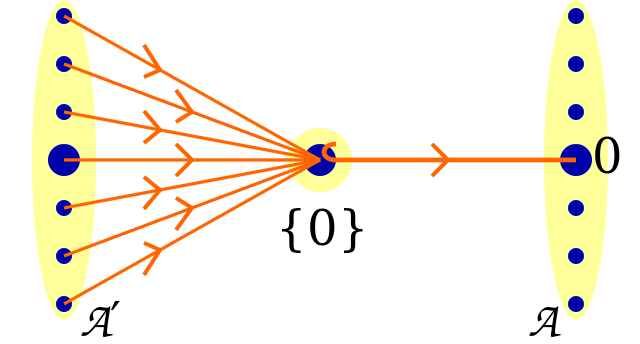
\includegraphics[scale=0.3]{img/01-obj.eps}
 %\captionsetup{labelformat=empty}
 \caption{零对象}
 \label{fig:zero-obj}
\end{figure}

平凡群中唯一的元素是什么名字不重要,它可以是$e$,可以是1(例如整数乘法群的平凡子群),可以是0(例如整数加群的平凡子群),可以是$I$(例如方阵乘法群中的单位矩阵),可以是(1)(置换群中的恒等置换),可以是$id$……在同构的意义下它们都是等价的。
\end{example}

\begin{example}
现在我们把难度增加一点,考虑全体集合的范畴$\pmb{Set}$,箭头是全函数。终止对象相对容易找到,就是只含有一个元素的集合(singleton)$\{ \bigstar \}$。仿照群的例子,对于任何集合$S$,我们让集合中所有的元素都映射到这个唯一的元素上去:$\forall x \in S, x \mapsto \bigstar$。显然这个箭头是唯一的。

\[
  S \longrightarrow \{ \bigstar \}
\]

但是问题来了,空集$\varnothing$怎样映射到$\{ \bigstar \}$上?事实上,空集是集合范畴中的起始对象。对于任何集合$S$,我们都可以定义箭头

\[
  \varnothing \arrowto{f} S
\]

这一点比较难理解,请停下来仔细思考一下。可以从空集的$id$箭头出发思考这个问题,$\varnothing \arrowto{id_{\varnothing}} \varnothing$。根据范畴公理,$id$箭头是任何范畴中任何对象都有的。空集是到任何集合(包括它自己)都存在唯一箭头的对象。只不过这个箭头所表示的全函数没有任何参数。它不能写成$f(x): x \mapsto y$的形式。

回答刚才的问题,由于空集到任何集合都有唯一的箭头,所以空集到$\{ \bigstar \}$也有唯一的箭头。这样从任何集合(包括空集)都存在到$\{ \bigstar \}$的唯一箭头,因此$\{ \bigstar \}$的确是集合范畴中的终止对象。

为什么不能像群一样,让只含有一个元素的集合$\{ \bigstar \}$成为起始对象呢?原因是,从$\{ \bigstar \}$到任意集合$S$的箭头可能不唯一。考虑有若干元素的集合$S = \{x, y, z, ...\}$,我们可以定义箭头(全函数)$\{ \bigstar \} \arrowto{\vec{x}} S$,将唯一元素映射到$x$上,也可以定义箭头$\{ \bigstar \} \arrowto{\vec{y}} S$和$\{ \bigstar \} \arrowto{\vec{z}} S$,将其映射到其它元素上。

我们选择符号$\{ \bigstar \}$的用意是说,元素是什么不重要,只要它是只含有一个元素的集合(singleton set),在同构意义上就是等价的。

\label{sec:selection-arrow} \index{选择箭头}
从终止对象$\{ \bigstar \}$到某一集合$S$的箭头

\[
  \{ \bigstar \} \longrightarrow S
\]

也有着特定的含义。它表明我们可以从集合$S$中选出一个元素,例如上述的箭头$\vec{x}$,从集合中选出元素$x$。我们把这样的箭头叫做\textbf{选择箭头}。
\end{example}

\begin{example}
在最后一个例子中,我们来到编程领域。编程环境的类型系统本质上是集合范畴$\pmb{Set}$。一个集合相当于是一个数据类型。例如整形$Int$是所有整数的集合;布尔型是两个元素$\{True, False\}$组成的集合。既然集合范畴的终止对象是$\{ \bigstar \}$,那么什么数据类型是编程中的终止对象呢?由于终止对象在同构的意义下是唯一的,所以任何只含有一个值的数据类型都是编程中的终止对象。

例如在Haskell中,特别定义了一个数据类型叫做“()”,它只含有一个元素,也叫做“()”。

\begin{lstlisting}
data  ()  =  ()
\end{lstlisting}

在同构的意义下$\{ \bigstar \} = \{()\}$,我们稍后会看到用“()”的好处。可以这样定义所有类型(集合)到这个终止对象的箭头(全函数):

\begin{lstlisting}
unit :: a -> ()
unit _ = ()
\end{lstlisting}

我们也可以自己定义终止对象——任何只有一个值的数据类型,在同构的意义上它和()是等价的\footnote{在其它编程环境,例如C++, Java,Scala中,可以定义“单子”(Single)对象,如果把强制类型转换作为箭头,则这也构成了终止对象。}。

\begin{lstlisting}
data Singleton = S

proj :: a -> Singleton
proj _ = S
\end{lstlisting}

看起来这像一个常函数,把任何值都映射到一个常数的值,但是并非所有常函数都指向终止对象,例如下面两个常函数:

\begin{lstlisting}
yes :: a -> Bool
yes _ = True

no :: a -> Bool
no _ = False
\end{lstlisting}

因为数据类型$Bool$包含两个元素,所以任何其他数据类型都有$yes, no$两个箭头指向$Bool$,这样就不满足终止对象箭头的唯一性要求。

在集合范畴中,起始对象是空集$\varnothing$,那么在编程中它对应着什么数据类型呢?既然数据类型本质上是集合,那么空集就相当于没有任何值的数据类型。在编程中,相当于我们声明了一个数据类型,但是却没有对它进行定义。

例如在Haskell中,声明了一个类型\texttt{Void},但是却没有为它定义任何值:

\begin{lstlisting}
data Void
\end{lstlisting}

这样\texttt{Void}就表示一个空集。但是起始对象必须有到所有其它对象的唯一箭头。这就要求我们必须定义从\texttt{Void}到所有其他类型的函数。

\begin{lstlisting}
absurd :: Void -> a
absurd _ = undefined
\end{lstlisting}

函数的具体实现并不重要,因为根本不存在一个实际的参数来调用这个函数。因此在Haskell标准库的某个版本中还有这样的实现:

\begin{lstlisting}
absurd :: Void -> a
absurd a = case a of {}
\end{lstlisting}

我们也可以自己定义起始对象,只要在同构的意义上是等价的就可以。方法就是只声明类型,不定义任何值。例如:

\begin{lstlisting}
data Empty

f :: Empty -> a
f _ = undefined

iso :: Void -> Empty
iso _ = undefined

iso' :: Empty -> Void
iso' _ = undefined
\end{lstlisting}

我们明确定义了$iso$和$iso'$,使得\texttt{Empty}和$\texttt{Void}$是同构的。并且容易验证\texttt{iso . iso' = id}。

集合范畴的例子中,我们说从终止对象到任何集合的箭头叫做选择箭头,它在编程中意味着什么呢?集合对应着类型,它表示我们可以从任何类型中选出特定的值。例如下面的函数从$Int$中分别选出0和1:

\begin{lstlisting}
zero :: () -> Int
zero () = 0

one :: () -> Int
one () = 1
\end{lstlisting}

现在我们看到用“()”的好处了,调用的时候,就像传入0个参数的函数那样:$zero\ ()$返回0,$one\ ()$返回1。
\end{example}

\begin{Exercise}
\Question{在本节的例子中,我们说在一个偏序集中,如果存在最小值(或最大值),则最小值(或最大值)就是起始对象(或终止对象)。考虑全体偏序集构成的范畴$\pmb{Poset}$,如果存在起始对象,它是什么?如果存在终止对象,它是什么?}
\Question{皮亚诺范畴$\pmb{Pno}$(参见本章第一节的习题2)中,什么样的对象$(A, f, z)$是起始对象?终止对象是什么?}
\end{Exercise}

\subsection{幂}

起始对象和终止对象,相当于0和1,积和余积相当于$\times$和$+$,如果再有了指数(幂),我们就可以在范畴这个抽象层面中拥有和基本算术运算,甚至和多项式“同构”的强大工具。

观察一个定义在自然数上二元函数$f(x, y) = z$,例如$f(x, y) = x^2 + 2y + 1$。其类型为$f: N \times N \to N$。我们会自然联想到,可以把这个类型写成:

\[
f : N^2 \to N
\]

对于函数$f$,我们能否把$N^2$看成一个对象,而不是两个参数呢?也就是说,看成$f\ (x, y)$,而不是$f(x, y)$。如果把参数看成一个“洞”,则前者是$f\ \bullet$,然后把一个对$(x, y)$填入洞中;而后者是$f(\bullet, \bullet)$,然后分别把$x, y$填入到两个洞中。另一方面,在第二章我们介绍了克里化,可以把$f$看成$f: N \to (N \to N)$,也就是传入$x$后,$f\ x$会返回另一个函数,这个新函数把一个自然数映射到另一个自然数。但使用克里化,我们反而得不到幂的概念了。峰回路转,如果我们把克里化后返回的东西,也就是$N \to N$看成一个事物,比方叫做“函数对象”会怎样呢?$N$是一个无穷集,想起来比较困难。我们后退一步,构造一个简单点的例子——只有两个元素的有限集$Bool$——来分析一下。

\begin{example}
存在无穷多个从$Bool$到$Int$的函数(箭头)组成的集合$\{Bool \arrowto{f} Int\}$,我们从这个集合中挑选一个元素,也就是一个例子函数来看看:

\[
\begin{array}{l}
ord : Bool \to Int \\
ord\ False = 0 \\
ord\ True = 1 \\
\end{array}
\]

它的结果是一对整数$(0, 1)$,这是一个代表,我们可以把所有上述箭头集合中的元素写成这样的形式:

\[
\begin{array}{l}
f : Bool \to Int \\
f\ False = ... \\
f\ True = ... \\
\end{array}
\]

不管$f$怎样千变万化,结果总是一对整数$(a, b)$。我们可以说箭头$f$的集合,同构于一对整数$(a, b)$的集合,即:

\[
\begin{array}{rcl}
\{Bool \arrowto{f} Int\} & = & \{(a = f\ False, b = f\ True)\} \\
  & = & Int \times Int \\
  & = & Int^2 = Int^{Bool}
\end{array}
\]

这告诉我们,箭头的集合,也就是箭头的类型\footnote{严格来说,我们应该去掉上面箭头两侧的大括号,增加大括号是为了容易理解}:$Bool \to Int$,相当于一个幂$Int^{Bool}$。也就是说$Bool \to Int = Int^{Bool}$。为什么在上面的推理中,我们可以用$Bool$替换$2$,从而把$Int^2$变成$Int^{Bool}$呢?原因是同构,上述的等号的真正含义是同构,所以严格来说,应该用“$\cong$”符号,而不是“=”。$Int^2$,是两个整数积的自然记法,也就是一对$Int$值的集合。一对$Int$值的集合可以看成是从一个名叫\textbf{2}的,拥有2个元素的索引集合$\{0, 1\}$到$Int$的映射。

\[
\{0, 1\} \arrowto{f} Int = \{(f(0), f(1))\} = Int^2
\]

而索引集合$\mathbf{2} = \{0, 1\}$正是$Bool$的同构(例如在$ord$函数下)。
\end{example}

\begin{example}
再举一个例子,考虑所有从字符$Char$到布尔值$Bool$的函数(箭头)集合$Char \to Bool$。这个集合里有很多函数,例如$isDigit(c)$可以判断传入的字符是否是数字。它可以实现为:

\lstset{frame=none}
\begin{lstlisting}[style=Haskell]
isDigit : Char -> Bool
...
isDigit '0' = True
isDigit '1' = True
...
isDigit '9' = True
isDigit 'a' = False
isDigit 'b' = False
...
\end{lstlisting}

虽然这个实现比较的笨拙,但是它反映了一个事实:如果$Char$中有256个不同的字符(例如英语ASCII码),则函数$isDigit$的结果本质上和一个256元组(False, ..., True, True, ... True, False, ...)同构。这个元组中对应数字字符的位置是True,其余是False。在$Char \to Bool$中的众多函数中,$isUpper$,$isLower$,$isWhitespace$等等分别对应一个特定的元组。例如$isUpper$对应的元组中,大写字符所在的位置上为True,其余为False。这样尽管有无穷多种方式来定义一个从$Char$到$Bool$的函数,但从结果上看,本质上只有$2^{256}$个不同的函数。也就是说$Char \to Bool$和256元组的布尔值集合$Bool^{Char}$同构。
\end{example}

现在我们把例子中的集合推进到无限集。在这一节的开头,我们说克里化后的函数$f: N \to (N \to N)$,是从自然数$N$到“函数对象”的函数。我们把函数对象记为$(\Rightarrow)$,则$f$的类型为$N \arrowto{f} (\Rightarrow)$。也就是从索引集$\{0, 1, ...\}$到$(\Rightarrow)$的映射,它是一个无穷长元组的集合,元组的每个值都是一个函数对象。记为$(\Rightarrow)^N$。

\index{apply}
一般来说,我们把函数的集合$f : B \to C$记为$C^B$。从这个集合中取出一个函数$f \in C^B$,然后在从集合$B$中取出一个值$b \in B$,我们可以用一个名叫$apply$的函数将$f$应用到$b$上,从而得到一个$C$中的值$c = f(b)$。即\footnote{有些文献,例如\cite{PeterSmith2018}第111-112页, \cite{Wiki-Exponentials}使用$eval$,也就是求值(evaluation)作为名称,这里采用和\cite{Bird97}(第72页)一致的命名。这样和Lisp中的命名传统一致。}:

\[
apply(f, b) = f(b)
\]

聪明的读者可能会问:符号$A$哪里去了?因为$A$还有别的用处。我们还要把克里化考虑进来。对于二元函数$g: A \times B \to C$,传入一个$A$中的值$a$后,就得到了一个克里化的函数$g(a, \bullet) : B \to C$。它是一个函数对象,属于$C^B$。这样,对于任何二元函数$A \times B \arrowto{g} C$,都存在唯一的一元函数$A \arrowto{\lambda g} C^B$,将$a \in A$送入$g(a, \bullet) : B \to C$中。我们称$\lambda g$为$g$的幂转换(exponential transpose)\footnote{有的文献中用$\bar{g}$来表示,根据第二章中对$\lambda$的介绍,以及关于丘奇出版商的小插曲,我认为用$\lambda g$更为传神,它表示$a \mapsto \lambda \bullet \cdot g(a, \bullet)$。}。并且,有这样的关系:


\[
apply(\lambda g(a), b) = g(a, b)
\]

也就是说,$apply$把一个类型为$C^B$的函数对象$\lambda g(a)$与类型为$B$的参数$b$组合在一起,最终得到类型为$C$的结果$c$。所以箭头$apply$的类型为:

\[
C^B \times B \arrowto{apply} C
\]

\index{幂对象(Expenentials或Expenential object)}
现在,我们终于可以给出完整的幂对象(Expenentials或Expenential object)定义了。

\begin{definition}
如果范畴$\pmb{C}$中存在终止对象和积,则一个\textbf{幂对象}是一对对象和箭头

\[
(C^B, apply)
\]

它们满足对于任何的对象$A$和箭头$A \times B \arrowto{g} C$,都存在唯一的转换箭头

\[
 A \arrowto{\lambda g} C^B
\]

使得下面的范畴图可交换

\begin{center}
\begin{tikzpicture}
  \matrix (m) [matrix of math nodes,
               row sep=3em, column sep=5em, minimum width=2em]{
     A & A \times B & \\
     C^B & C^B \times B & C \\};
  \path[-stealth]
    (m-1-1) edge node [left] {$\lambda g$} (m-2-1)
    (m-1-2) edge node [left] {$\lambda g \times id_B$} (m-2-2)
    (m-1-2) edge node [above] {$g$} (m-2-3)
    (m-2-2) edge node [below] {$apply$} (m-2-3);
\end{tikzpicture}
\end{center}

即:

\[
  apply \circ (\lambda g \times id_B) = g
\]

\end{definition}

\index{克里化}
第二章中我们没有给出克里化的完整定义,现在利用幂对象,我们可以给出$curry$的定义了:

\[
\begin{array}{l}
curry : (A \times B \to C) \to A \to (C^B) \\
curry\ g = \lambda g
\end{array}
\]

因此,$curry\ g$就是$g$的幂转换。把这一关系代入上面的范畴图,我们有:

\[
  apply \circ (curry\ g \times id) = g
\]

换言之,我们就得到了这样的泛性性质:

\[
  f = curry\ g \quad \equiv \quad apply \circ (f \times id) = g
\]

并且我们还能说明为什么幂转换箭头是唯一的,假设还存在另外的箭头$A \arrowto{h} C^B$,使得$apply \circ (h \times id) = g$,根据上述泛性性质,我们立刻得到$h = curry\ g$。

我们还可以从范畴的角度来理解幂对象,在范畴$\pmb{C}$中,如果固定对象$B, C$,我们可以构造一个名叫$\pmb{Exp}$的范畴,这个范畴中的对象是$A \times B \to C$这样的箭头,范畴中的箭头是这样定义的。

\begin{center}
\begin{tikzpicture}
  \matrix (m) [matrix of math nodes,
               row sep=3em, column sep=5em, minimum width=2em]{
     A & A \times B \arrowto{h} C \\
     D & D \times B \arrowto{k} C \\};
  \path[-stealth]
    (m-1-1) edge node [left] {$f$} (m-2-1)
    (m-1-2) edge node [left] {$j$} (m-2-2);
\end{tikzpicture}
\end{center}

如果在$\pmb{C}$中存在$A \arrowto{f} D$的箭头,则$\pmb{Exp}$中的箭头为$h \arrowto{j} k$。当且仅当把上面范畴图中右侧的$C$合并时,箭头之间可交换:

\begin{center}
\begin{tikzpicture}
  \matrix (m) [matrix of math nodes,
               row sep=3em, column sep=5em, minimum width=2em]{
     A & A \times B & \\
     D & D \times B & C \\};
  \path[-stealth]
    (m-1-1) edge node [left] {$f$} (m-2-1)
    (m-1-2) edge node [left] {$f \times id_B$} (m-2-2)
    (m-1-2) edge node [above] {$h$} (m-2-3)
    (m-2-2) edge node [below] {$k$} (m-2-3);
\end{tikzpicture}
\end{center}

即:$k \circ (f \times id_B) = h$。在这个范畴$\pmb{Exp}$中,存在一个终止对象,它恰好是$C^B \times B \arrowto{apply} C$。我们现在来验证一下,根据幂对象的定义,从任何其它对象$A \times B \arrowto{g} C$,都有到$apply$的箭头$\lambda g = curry\ g$。另外根据终止对象的性质,从终止对象到自己的箭头一定是$id$,所以我们有\textbf{反射律}:

\[
curry\ apply = id
\]

\begin{Exercise}
\Question{验证$\pmb{Exp}$的确是一个范畴,指出$id$箭头和箭头的组合。}
\Question{反射律$curray\ apply = id$中,$id$的下标是什么?请用另一种方法证明它。}
\Question{我们称下面的等式
\[
(curry\ f) \circ g = curry(f \circ (g \times id))
\]
为克里化的融合律。请画出它的范畴图并证明它。}
\end{Exercise}

\subsection{笛卡尔闭和对象算术}

有了起始对象0,终止对象1,余积代表的加法,积代表的乘法,再加上幂对象代表的指数幂,我们终于拥有了在范畴上进行运算甚至构造抽象多项式的能力。但是且慢,让我们停下来看一下这样能跑多远。正如第三章开头我们讲到的,必须时刻关注一个问题:“某一种抽象的适用范围有多大?什么情况下这一抽象会失效?”

\index{笛卡尔闭}
并非所有的范畴都有起始或终止对象,也并非所有的范畴都有幂对象。如果一个范畴存在有限积、对于任何对象$A$和$B$都存在幂$A^B$,我们称这样的范畴为\textbf{笛卡尔闭}的(Cartesian closed)。一个笛卡尔闭范畴必须包含:

\begin{enumerate}
\item 一个终止对象(1);
\item 任何一对对象都有积($\times$);
\item 任何一对对象都有幂($A^B$)
\end{enumerate}

我们既可以把终止对象1,想象成一个对象的零次幂:$A^0 = 1$,也可以把它想象成零个对象的积。非常幸运的是,编程时我们所在的范畴——集合和全函数组成的范畴是笛卡尔闭的。一个笛卡尔闭范畴可以作为简单类型$\lambda$-演算(simply typed lambda calculus)的数学模型(见第二章),从而成为所有带有类型的编程语言的基础(\cite{Milewski2018}第148页)。

\index{双笛卡尔闭(Bicartesian closed)}
如果一个笛卡尔闭的范畴还同时支持终止对象的对偶——起始对象,和积的对偶——余积。并且支持积和余积的分配律,我们称其为\textbf{双笛卡尔闭}范畴(Bicartesian closed):

\begin{enumerate}
  \setcounter{enumi}{4}
  \item 一个起始对象(0);
  \item 任何一对对象都有余积($+$);
  \item 积可以从左右两侧分配到余积上:
  \[
  \begin{array}{l}
  A \times (B + C) = A \times B + A \times C \\
  (B + C) \times A = B \times A + C \times A
  \end{array}
  \]
\end{enumerate}

\index{对象算术}
现在我们可以看看基本算术运算在一个笛卡尔闭的范畴上,特别是编程中都意味着什么了。这一理论称为对象算术理论(Equational theory)。

\subsubsection{0次幂}

\[
  A^0 = 1
\]

0代表了起始对象,1代表了终止对象,$A$的0次幂可以解读为类型为$0 \to A$的所有箭头的集合。但既然0是起始对象,所以它到任何对象只有唯一的箭头。因此集合$\{ 0 \to A \}$仅仅含有一个元素(singleton),而仅有一个元素的集合$\{ \bigstar \}$恰巧是(集合范畴的)终止对象1。下面的推导中等号应理解为同构。

\[
\begin{array}{rcll}
A^0 & = & \{ 0 \to A \} & \text{幂对象的定义} \\
    & = & \{ \bigstar \} & \text{起始对象到任何对象的箭头唯一} \\
    & = & 1 & \{ \bigstar \}\text{是终止对象} \\
\end{array}
\]

这样,算术中的任何数的0次幂等于1在范畴中也得到了解读。

\subsubsection{1的幂}

\[
  1^A = 1
\]

1代表了终止对象,所以幂对象$1^A$表示所有从$A$出发,到终止对象的箭头的集合$\{ A \to 1 \}$。根据终止对象的定义,任何对象到终止对象只有唯一的箭头,所以这个箭头集合仅仅含有一个元素,而仅有一个元素的集合同构于$\{ \bigstar \}$。它恰好又是(集合范畴中的)终止对象。

\[
\begin{array}{rcll}
1^A & = & \{ A \to 1 \} & \text{幂对象的定义} \\
    & = & \{ \bigstar \} & \text{任何对象到终止对象的箭头唯一} \\
    & = & 1 & \{ \bigstar \}\text{是终止对象} \\
\end{array}
\]

\subsubsection{1次幂}

\[
  A^1 = A
\]

这恰好是前面介绍过的“\hyperref[sec:selection-arrow]{选择箭头}”。1是终止对象,所以幂$A^1$表示了从终止对象到$A$的箭头集合$\{ 1 \to A\}$。如果$A$是一个集合,我们可以针对集合中的任何元素$a \in A$构造一个从终止对象1到$a$的一个函数:

\[
  f_a : 1 \to a
\]

这种选择函数,能从集合$A$中选出一个元素$a$。所有从1到$A$中元素的选择函数的集合为$\{f_a : 1 \mapsto a | a \in A\}$,它恰好就是集合$1 \to A$。另一方面,集合$\{ f_a \}$是和$A = \{a\}$一一对应的,也就是说它们是同构的。

\[
\begin{array}{rcll}
A^1 & = & \{ 1 \to A \} & \text{幂对象的定义} \\
    & = & \{ f_a : 1 \mapsto a | a \in A \} & \text{从1到$A$中元素的映射的集合} \\
    & = & \{ a | a \in A \} = A & \text{一一映射同构} \\
\end{array}
\]

\subsubsection{幂的和}

\[
  A^{B + C} = A^B \times A^C
\]

幂对象$A^{B + C}$表示从余积$B + C$到$A$的箭头的集合$\{B + C \to A\}$。我们借助$\mathbf{Either}\ B\ C$来帮助我们思考\footnote{也可以用标记(tag)来推理:
\[
\begin{array}{l}
f : B + C \to A \\
f (b, 0) = ... \\
f (c, 1) = ...
\end{array}
\]
},当我们实现任何$\mathbf{Either}\ B\ C \to A$函数时,都可以写成这样的形式:

\[
\begin{array}{l}
f : \mathbf{Either}\ B\ C \to A \\
f\ left\ b = ... \\
f\ right\ c = ... \\
\end{array}
\]

也就是说,任何这样的函数,都可以看作一对映射$(b \mapsto a_1, c \mapsto a_2)$,而$\{(b \mapsto a_1, c \mapsto a_2)\}$恰好是$B \to A$和$C \to A$的积。因此$\{B + C \to A\} = \{B \to A\} \times \{C \to A\}$。另一方面,根据$\{B \to A\}$可以表示为幂对象$A^B$,同样$\{C \to A\}$可以表示为$A^C$。这样就解读了幂的和:

\[
\begin{array}{rcll}
A^{B + C} & = & \{ B + C \to A \} & \text{幂对象的定义} \\
    & = & \{ (b \mapsto a_1,  c \mapsto a_2) | a_1, a_2 \in A, b \in B, c \in C\} & \text{$B$和$C$到$A$的箭头对} \\
    & = & \{ B \to A \} \times \{ C \to A \} & \text{笛卡尔积} \\
    & = & A^B \times A^C & \text{幂对象} \\
\end{array}
\]

\subsubsection{幂的幂}

\[
  (A^B)^C = A^{B \times C}
\]

先看右侧,幂对象$A^{B \times C}$实际就是二元函数$B \times C \arrowto{g} A$的集合。交换积的次序$C \times B \arrowto{g \circ swap} A$,显然是一个自然同构(参见自然同构一节的$swap$自然变换)。如果克里化,就是$\{curry(g \circ swap)\} = \{C \to A^B\}$,再一次用幂对象表示就是$(A^B)^C$。

\[
\begin{array}{rcll}
A^{B \times C} & = & \{B \times C \arrowto{g} A \}  & \text{幂对象的定义} \\
    & = & \{ C \times B \arrowto{g \circ swap} A \} & \text{自然同构} \\
    & = & \{ C \arrowto{curry(g \circ swap)} A^B \} & \text{克里化后仍然同构} \\
    & = & (A^B)^C & \text{幂对象} \\
\end{array}
\]

\subsubsection{积的幂}

\[
  (A \times B)^C = A^C \times B^C
\]

幂对象$(A \times B)^C$是箭头$C \to A \times B$的集合,它可以认为是返回一对值的函数集合$\{ c \mapsto (a, b)\}$,其中$c \in C, a \in A, b \in B$。它显然同构于$\{(c \mapsto a, c \mapsto b)\}$,而这恰恰是箭头$C \to A$和$C \to B$的积。最后再分别将$C \to A$和$C \to B$表示为幂对象就得到了幂的积。

\[
\begin{array}{rcll}
(A \times B)^C & = & \{C \to A \times B \}  & \text{幂对象的定义} \\
    & = & \{ c \mapsto (a, b) | a \in A, b \in B, c \in C\} & \text{箭头的集合} \\
    & = & \{ (c \mapsto a, c \mapsto b) \} & \text{箭头对} \\
    & = & \{C \to A\} \times \{C \to B\} & \text{笛卡尔积} \\
    & = & A^C \times B^C & \text{幂对象} \\
\end{array}
\]

\subsection{多项式函子}
\label{sec:polynomial-functors}
\index{多项式函子}

以上介绍的在笛卡尔闭范畴上的算术主要是针对对象的。如果我们把函子考虑进来,会怎样呢?由于函子既作用于对象,也作用于箭头,这样就产生了多项式函子的概念。多项式函子是使用常函子(参见\hyperref[sec:functor:examples]{函子的例子中的“黑洞”函子})、积函子和余积函子递归构造的。

\begin{itemize}
  \item 恒等函子$id$和常函子$\mathbf{K}_A$是多项式函子;
  \item 若函子$\mathbf{F}$和$\mathbf{G}$是多项式函子,则它们的组合$\mathbf{FG}$,和$\mathbf{F} + \mathbf{G}$与积$\mathbf{F} \times \mathbf{G}$也是多项式函子。其中和与积定义如下:
  \[
    \begin{array}{l}
    (\mathbf{F} + \mathbf{G}) h = \mathbf{F} h + \mathbf{G} h \\
    (\mathbf{F} \times \mathbf{G}) h = \mathbf{F} h \times \mathbf{G} h \\
    \end{array}
  \]
\end{itemize}

举一个例子,若函子$\mathbf{F}$对于对象和箭头的行为是:

\[
\begin{cases}
\text{对象:} & \mathbf{F} X = A + X \times A \\
\text{箭头:} & \mathbf{F} h = id_A + h \times id_A
\end{cases}
\]

其中$A$是某个固定的对象。则函子$\mathbf{F}$是一个多项式函子。这是因为它可以表达为多项式:

\[
\mathbf{F} = \mathbf{K}_A + (id \times \mathbf{K}_A)
\]

\subsection{F-代数}

为了构造复杂的带有递归结构的代数数据类型,我们还需要最后一块砖石。这就是F-代数(F-algebras)。观察抽象代数中的概念,如幺半群、群、环、域,它们不仅仅是抽象的对象,而且带有结构。正是这些结构之间的关系,使得它们区别于过去那些具体的对象,例如数、点、线、面。如果关系和结构研究清楚了,不仅仅是数、点、线、面,所有具有同样关系和结构的对象(用希尔伯特的比喻,连同桌子、椅子、啤酒杯)就都尽在掌握了。

\begin{example}
我们从比较简单的幺半群作为开始的例子,一步一步导出F-代数的概念。一个幺半群是一个集合$M$,并且在集合上定义了可结合的二元运算和单位元。

如果用$\oplus$表示二元运算,$1_M$表示单位元,则幺半群的两条公理可以描述如下:

\[
\begin{cases}
\text{结合性公理:} & (x \oplus y) \oplus z = x \oplus (y \oplus z), \forall x, y, z \in M \\
\text{单位元公理:} & x \oplus 1_M = 1_M \oplus x = x, \forall x \in M \\
\end{cases}
\]

第一步,我们将二元运算$\oplus$表示为函数,将$1_M$表示为选择函数,定义:

\[
\begin{cases}
m (x, y) = x \oplus y \\
e () = 1_M
\end{cases}
\]

这两种箭头的类型分别为:

\[
\left \{
\begin{array}{lll}
 & \text{类型} & \text{幂对象} \\
\text{二元运算:} & M \times M \to M & M^{M \times M}\\
\text{选择运算:} & 1 \to M & M^1 \\
\end{array}
\right .
\]

第一种箭头是说,两个幺半群的元素进行二元运算,其结果仍是这个幺半群中的元素(二元运算是封闭的);第二种箭头是“选择函数”,1是终止对象\footnote{我们借鉴Haskell中的符号,特意用“()”表示终止对象,在同构的意义下$1 = \{ \bigstar \} = \{ () \}$。这样的好处是,$e()$看起来像是个无参数的函数调用,实际接受了终止对象中的唯一元素()作为参数。}。

现在我们就可以用函数$m$和$e$来替换幺半群公理了:

\[
\begin{cases}
\text{结合性公理:} & m(m(x, y), z) = m(x, m(y, z)), \forall x, y, z \in M \\
\text{单位元公理:} & m(x, e()) = m(e(), x) = x, \forall x \in M \\
\end{cases}
\]

第二步,把所有的$x, y, z$等具体的元素和对象$M$都去掉。这样就得到了纯用函数(箭头)表示的幺半群公理:

\[
\begin{cases}
\text{结合性公理:} & m \circ (m, id) = m \circ (id, m) \\
\text{单位元公理:} & m \circ (id, e) = m \circ (e, id) = id \\
\end{cases}
\]

这两条公理意味着下面的两个范畴图中的箭头可交换:

\begin{figure}[htbp]
\centering
\subcaptionbox{结合性公理}{\subimport{img/}{monoid-assoc.tex}}
\quad
\subcaptionbox{单位元公理}{\subimport{img/}{monoid-e.tex}}
\caption{幺半群公理对应的范畴图}
\end{figure}

现在可以说,任何幺半群都可以用一个三元组$(M, m, e)$来表示了。其中$M$是集合,$m$是二元运算函数,$e$是单位元选择函数。

第三步,$(M, m, e)$不仅规定了幺半群的集合,还规定了在此集合上的二元运算和单位元,因此整个幺半群的代数结构就都确定了。组成幺半群的所有箭头,也就是代表所有可能的$m$和$e$的箭头集合,是两种幂对象的积

\[
M^{M \times M} \times M^1 = M^{M \times M + 1}
\]

我们再把右侧从幂对象写回箭头的形式,这样集合$M$上定义的幺半群代数运算一定是下面的形式:

\[
\begin{array}{rcll}
\alpha : 1 + M \times M & \longrightarrow & M & \text{和(余积)}\\
1 & \longmapsto & 1 & \text{单位元}  \\
(x, y) & \longmapsto & x \oplus y & \text{二元运算}
\end{array}
\]

通过余积用和来表示这种关系就是$\alpha = e + m$,用多项式函子来表示就是$\mathbf{F} M = 1 + M \times M$

总结一下,对于幺半群这个例子,幺半群上的代数结构由三部分组成:

\begin{enumerate}
  \item 对象$M$,就是用于携带幺半群上代数结构的集合,叫做\textbf{携带对象}(carrier object);
  \item 函子$\mathbf{F}$,定义了幺半群上的代数运算。是一个多项式函子$\mathbf{F} M = 1 + M \times M$;
  \item 箭头$\mathbf{F} M \arrowto{\alpha} M$,它是单位元箭头$e$和二元运算箭头$m$的和(余积),$\alpha = e + m$。
\end{enumerate}

我们称这样定义了一个幺半群的$F$-代数$(M, \alpha)$。

例如在Haskell中,可以这样定义一个F-代数箭头的类型:

\begin{lstlisting}
type Algebra f a = f a -> a
\end{lstlisting}

这本质上是给箭头$\mathbf{F}A \to A$起了一个别名(alias),名叫\texttt{Algebra} $\mathbf{F}, A$。对于幺半群,还需要定义一个函子\footnote{
Haskell中有一个对幺半群的标准定义(见本章附录)。但这是一个幺半群代数结构的定义,而不是幺半群函子。}:

\begin{lstlisting}
data MonoidF a = MEmptyF | MAppendF a a
\end{lstlisting}

当\texttt{a}是字符串时,我们可以这样定义一个F-代数\texttt{(String, evals)}的箭头实现:

\begin{lstlisting}
evals :: Algebra MonoidF String
evals MEmpty = e ()
evals (MAppendF s1 s2) = m s1 s2

e :: () -> String
e () = ""

m :: String -> String -> String
m = (++)
\end{lstlisting}

当然,也可将\texttt{e}和\texttt{m}内嵌到\texttt{evals}中简化实现为:

\begin{lstlisting}
evals :: Algebra MonoidF String
evals MEmpty = ""
evals (MAppendF s1 s2) = s1 ++ s2
\end{lstlisting}

\texttt{evals}是箭头$\alpha : \mathbf{F}A \to A$的一种实现,其中$\mathbf{F}$为\texttt{MonoidF},$A$为\texttt{String}。当然还可以有别的实现,只要它能够满足幺半群的单位元公理和结合性公理。
\end{example}

\begin{example}
在幺半群之上,增加一条可逆性公理,就得到了群。我们仍然分步骤引出群的F-代数。首先列出群元素集合$G$上的三条公理,我们用$1_G$表示单位元,点号表示二元运算,$()^{-1}$表示求逆元:

\[
\begin{cases}
\text{结合性公理:} & (x \cdot y) \cdot z = x \cdot (y \cdot z), \forall x, y, z \in G \\
\text{单位元公理:} & x \cdot 1_G = 1_G \cdot x = x, \forall x \in G \\
\text{可逆性公理:} & x \cdot x^{-1} = x^{-1} \cdot x = 1_G, \forall x \in G
\end{cases}
\]

第一步,将二元运算,求单位元、求逆元都表示为函数。定义:

\[
\begin{cases}
m (x, y) = x \cdot y \\
e () = 1_G \\
i (x) = x^{-1}
\end{cases}
\]

这三种函数的类型和幂对象分别为:

\[
  \left \{
    \begin{array}{lll}
      \text{二元运算:} & G \times G \to G & G^{G \times G}\\
      \text{选择运算:} & 1 \to G & G^1 \\
      \text{求逆运算:} & G \times G & G^G \\
    \end{array}
  \right . \\
\]

前两个箭头和幺半群一样,第三个箭头是说群元素的逆元仍是群中的元素。现在就可以用$e, m ,i$替换群公理中的$1_G$,点号和逆元符号了。

\[
\begin{cases}
\text{结合性公理:} & m(m(x, y), z) = m(x, m(y, z)), \forall x, y, z \in G \\
\text{单位元公理:} & m(x, e()) = m(e(), x) = x, \forall x \in G \\
\text{可逆性公理:} & m(x, i(x)) = m(i(x), x) = e(), \forall x \in G \\
\end{cases}
\]

第二步,把所有的具体元素$x, y, z$和群元素集合$G$去掉。得到纯用箭头表示的群公理:

\[
\begin{cases}
\text{结合性公理:} & m \circ (m, id) = m \circ (id, m) \\
\text{单位元公理:} & m \circ (id, e) = m \circ (e, id) = id \\
\text{可逆性公理:} & m \circ (id, i) = m \circ (i, id) = e \\
\end{cases}
\]

这样,任何群都可以用一个四元组$(G, m, e, i)$表示。

第三步,利用余积求$m, e, i$的和$\alpha = e + m + i$,通过多项式函子$\mathbf{F} A = 1 + A + A \times A$,并令$A = G$,描述群$G$上的代数运算。

\[
\begin{array}{rcll}
\alpha : 1 + A + A \times A & \longrightarrow & A & \text{和(余积)}\\
1 & \longmapsto & 1 & \text{单位元}  \\
x & \longmapsto & x^{-1} & \text{逆元} \\
(x, y) & \longmapsto & x \cdot y & \text{二元运算} \\
\end{array}
\]

所以,群上的代数结构由三部分组成:

\begin{enumerate}
  \item 携带对象$G$,用于携带群上代数结构的集合;
  \item 多项式函子$\mathbf{F} A = 1 + A + A \times A$,定义了群上的代数运算;
  \item 箭头$\mathbf{F} A \arrowto{\alpha = e + m + i} A$,它是单位元箭头$e$、二元运算箭头$m$、逆元箭头$i$的和。
\end{enumerate}

我们称这样定义了一个群上的F-代数$(G, \alpha)$。
\end{example}

\index{F-代数} \index{F-余代数}
现在我们可以给出F-代数的定义了。在范畴论中,许多概念是对偶的,成对出现的。这就像是买一送一,我们定义了F-代数,就同时得到了F-余代数(F-coalgebra)\footnote{也译作上代数和共代数。}。关于F-余代数,我们暂时只给出定义。稍后将在第6章介绍无穷的概念时,再给出相应的例子。

\begin{definition}
如果$\pmb{C}$是一个范畴,$\pmb{C} \arrowto{\mathbf{F}} \pmb{C}$是范畴$\pmb{C}$上的一个自函子。对于范畴中的对象$A$和态射$\alpha$:

\[
  \mathbf{F} A \arrowto{\alpha} A
  \quad \quad \quad
  A \arrowto{\alpha} \mathbf{F} A
\]

构成一对元组$(A, \alpha)$叫做

\begin{center}
  F-代数 \quad \quad \quad F-余代数
\end{center}

其中$A$,叫做携带对象。

\end{definition}

我们可以把

\begin{center}
  F-代数$(A, \alpha)$ \quad \quad \quad F-余代数$(A, \alpha)$
\end{center}

本身看成对象。在上下文清楚的情况下,我们通常用二元组$(A, \alpha)$表示对象。
两个对象间的箭头定义如下:

\begin{definition}
F-态射是F-代数或F-余代数对象间的箭头:

\[
  (A, \alpha) \longrightarrow (B, \beta)
\]

如果携带对象间的箭头$A \arrowto{f} B$,使得下面的范畴图可交换:

\begin{center}
\begin{tikzpicture}
  \matrix (m) [matrix of math nodes,
               row sep=3em, column sep=3em, minimum width=2em]{
    \mathbf{F} A  & A &  & A & \mathbf{F} A \\
    \mathbf{F} B  & B &  & B & \mathbf{F} B \\};
  \path[-stealth]
    % left
    (m-1-1) edge node [above] {$\alpha$} (m-1-2)
    (m-1-1) edge node [left] {$\mathbf{F}(f)$} (m-2-1)
    (m-1-2) edge node [right] {$f$}   (m-2-2)
    (m-2-1) edge node [below] {$\beta$} (m-2-2)
    % right
    (m-1-4) edge node [above] {$\alpha$} (m-1-5)
    (m-1-4) edge node [left] {$f$} (m-2-4)
    (m-1-5) edge node [right] {$\mathbf{F}(f)$}   (m-2-5)
    (m-2-4) edge node [below] {$\beta$} (m-2-5);
\end{tikzpicture}
\end{center}

即:

\[
  f \circ \alpha = \beta \circ \mathbf{F}(f)
  \quad \quad \quad
  \beta \circ f = \mathbf{F}(f) \circ \alpha
\]
\end{definition}

F-代数和F-态射,F-余代数和F-态射分别构成了

\begin{center}
  F-代数范畴$\pmb{Alg}(\mathbf{F})$ \quad \quad \quad
  F-余代数范畴$\pmb{CoAlg}(\mathbf{F})$
\end{center}

\begin{Exercise}
\Question{画出群的可逆性公理的范畴图。}
\Question{$p$是一个素数,使用群的F-代数,为整数模$p$乘法群(可以参考上一章)定义一个$\alpha$箭头。}
\Question{参考上一章环的定义,定义环的F-代数。}
\Question{F-代数范畴上的$id$箭头是什么?箭头组合是什么?}
\end{Exercise}

\subsubsection{递归和不动点}

在第一章中,我们介绍了自然数和皮亚诺公理。并且介绍了和自然数同构的事物。实际上,我们可以把所有类似自然数的东西都用F-代数描述。

假设有一个集合$A$,具有自然数的代数结构。例如第一章中介绍过的斐波那契数列,其中$A$是数对$(Int, Int)$。起始对象是$(1, 1)$,后继函数是$h(m, n) = (n, m + n)$。

为了用F-代数描述这一\textbf{类}代数结构,我们需要三样东西:函子,携带对象和$\alpha$箭头。根据皮亚诺公理,自然数的函子应当这样定义:

\lstset{frame=none}
\begin{lstlisting}
data NatF A = ZeroF | SuccF A
\end{lstlisting}

这个函子是一个多项式函子$\mathbf{NatF} A = 1 + A$。现在我们提出一个问题。如果令$A’ = \mathbf{NatF} A$,将其代入$\mathbf{NatF}$函子,那么$\mathbf{NatF} A'$是什么?应该是两重函子$\mathbf{NatF}(\mathbf{NatF} A)$。我们还可以重复这一过程得到三重的$\mathbf{NatF}(\mathbf{NatF}(\mathbf{NatF} A))$。我们可以重复无穷多次,现在我们给重复无穷多次后产生类型$\mathbf{NatF}(\mathbf{NatF}(...))$起名为$\mathbf{Nat}$,即:

\[
\begin{array}{rcll}
\texttt{data}\ \mathbf{Nat} & = & \mathbf{NatF}(\mathbf{NatF}(...)) & \text{无穷重} \\
         & = & ZeroF\ |\ SuccF\ (SuccF (...)) & \text{无穷重}SuccF \\
         & = & ZeroF\ |\ SuccF\ \mathbf{Nat} & \text{无穷重}SuccF\text{的类型是}\mathbf{Nat} \\
         & = & Zero\ |\ Succ\ \mathbf{Nat} & \text{重命名}
\end{array}
\]

这恰恰是我们在第一章定义的自然数类型。我们把\texttt{Nat}和\texttt{Nat A}并列写在一起:

\begin{lstlisting}
data Nat = Zero | Succ Nat

data NatF A = ZeroF | SuccF A
\end{lstlisting}

这是函子层面的递归,在第二章中,我们曾经遇到过类似的概念。将自函子应用到自身无穷次产生了\textbf{不动点}:

\[
\mathbf{Fix}\ \mathbf{F} = \mathbf{F}\ (\mathbf{Fix}\ \mathbf{F})
\]

自函子$\mathbf{F}$的不动点是$\mathbf{Fix}\ \mathbf{F}$,将$\mathbf{F}$应用到不动点上,得到的仍然是不动点。因此,$\mathbf{Nat}$是函子$\mathbf{NatF}$的不动点。也就是说$\mathbf{Nat} = \mathbf{Fix}\ \mathbf{NatF}$。

%% \[
%% \begin{array}{l}
%% fix : \mathbf{F}\ (\mathbf{Fix}\ \mathbf{F}) \to \mathbf{Fix}\ \mathbf{F} \\
%% fix\ \mathbf{F} = let\ \mathbf{X} = \mathbf{F} \mathbf{X}\ in\ \mathbf{X} \\
%% \\
%% unfix : (\mathbf{Fix}\ \mathbf{F}) \to \mathbf{F}\ (\mathbf{Fix}\ \mathbf{F}) \\
%% unfix\ (\mathbf{Fix}\ \mathbf{X}) = \mathbf{X} \\
%% \end{array}
%% \]

\begin{Exercise}
\Question{可否把类自然数函子写成如下递归的形式?谈谈你的看法。
\begin{lstlisting}
data NatF A = ZeroF | SuccF (NatF A)
\end{lstlisting}
}
\Question{我们可以为$\mathbf{NatF} Int \to Int$定义一个$\alpha$箭头,名叫$eval$:
\[
\begin{array}{l}
eval : \mathbf{NatF} Int \to Int \\
eval\ ZeroF = 0 \\
eval\ (SuccF\ n) = n + 1 \\
\end{array}
\]
如果迭代地将$A' = \mathbf{NatF} A$代入$\mathbf{NatF}$函子$n$次。我们把这样得到的函子记为$\mathbf{NatF}^n A$。试思考能否定义下面的$\alpha$箭头:
\[
\begin{array}{l}
eval : \mathbf{NatF}^n Int \to Int \\
\end{array}
\]
}
\end{Exercise}

\subsubsection{初始代数和向下态射}

在F-代数组成范畴$\pmb{Alg}(F)$中,如果存在初始对象,它会有什么特殊的性质呢?初始对象到其它对象的唯一箭头表示什么样的关系呢?F-代数范畴中的所有对象可表示为二元组$(A, \alpha)$,我们用类自然数的F-代数来举例。在$\pmb{Alg}(\mathbf{NatF})$中,所有的对象都表示为$(A, \alpha)$。其中$\mathbf{NatF}$的定义如同上小节;携带对象是$A$,箭头是$\mathbf{NatF} A \arrowto{\alpha} A$。

%% 例如$\mathbf{NatF}-alg(N, [zero, succ])$是一个F-代数对象,其中$zero, succ$的定义为:

%% \[
%% \begin{cases}
%% zero() = 0 \\
%% succ(n) = n + 1 \\
%% \end{cases}
%% \]

%% 它们的余积$\alpha = [zero, succ] = zero + succ$,也就是说:

%% \[
%% \begin{array}{l}
%% [zero, succ] : \mathbf{NatF} N \to N \\
%% [zero, succ]\ ZeroF = zero() \\
%% [zero, succ]\ (SuccF\ n) = succ(n) \\
%% \end{array}
%% \]

例如$(Int \times Int, fib)$是一个F-代数对象。其中携带对象是整数的积,箭头$\mathbf{NatF} (Int \times Int) \arrowto{fib} (Int \times Int)$的定义为:

\[
\begin{array}{l}
fib : \mathbf{NatF} (Int \times Int) \to (Int \times Int) \\
fib\ ZeroF = (1, 1) \\
fib\ (SuccF\ (m, n)) = (n, m + n) \\
\end{array}
\]

这是一种紧凑的定义。我们可以把它也写成和(余积)的形式$fib = [start, next]$,其中$start$总返回$(1, 1)$,而$next(m, n) = (n, m + n)$。

如果范畴$\pmb{NatF}$有起始对象0,我们把它表示为二元组$(I, i)$。起始对象到任何对象$(A, \alpha)$都有唯一的箭头。即存在箭头$I \arrowto{f} A$,使得下面的范畴图可交换\footnote{起始的英文是initial,所以选择符号$(I, i)$代表起始对象中的集合$I$和箭头$i$}:

\begin{center}
\begin{tikzpicture}
  \matrix (m) [matrix of math nodes,
               row sep=3em, column sep=3em, minimum width=2em]{
    \mathbf{NatF} A  & A \\
    \mathbf{NatF} I  & I \\};
  \path[-stealth]
    (m-1-1) edge node [above] {$\alpha$} (m-1-2)
    (m-2-1) edge node [left] {$\mathbf{NatF}(f)$} (m-1-1)
    (m-2-2) edge node [right] {$f$}   (m-1-2)
    (m-2-1) edge node [below] {$i$} (m-2-2);
\end{tikzpicture}
\end{center}

因为起始对象到\textbf{任何}对象都有唯一箭头,所以它到自己的递归——由$\mathbf{NatF}(\mathbf{NatF}I)$——构成的对象也一定有唯一的箭头。具体来说这个递归的F-代数具有的三要素是:

\begin{enumerate}
\item 共同的函子$\mathbf{NatF}$;
\item 携带对象是$\mathbf{NatF}I$;
\item 箭头$\mathbf{NatF}(\mathbf{NatF}I) \to \mathbf{NatF}I$。因为函子既作用于对象,也作用于箭头。所以我们可以通过函子$\mathbf{NatF}$,将初始对象中的箭头$i$“举”上去。因此,这个递归的F-代数的箭头就是$\mathbf{NatF}(i)$。
\end{enumerate}

这样,这个递归的F-代数可以记为:$(\mathbf{NatF}I, \mathbf{NatF}(i))$。因为从初始对象到它也有唯一的箭头,所以存在$I \arrowto{j} \mathbf{NatF}I$,使得下面的范畴图可交换:

\begin{center}
\begin{tikzpicture}
  \matrix (m) [matrix of math nodes,
               row sep=3em, column sep=3em, minimum width=2em]{
    \mathbf{NatF}(\mathbf{NatF} I)  & \mathbf{NatF} I \\
    \mathbf{NatF} I  & I \\};
  \path[-stealth]
    (m-1-1) edge node [above] {$\mathbf{NatF}(i)$} (m-1-2)
    (m-2-1) edge node [left] {$\mathbf{NatF}(j)$} (m-1-1)
    (m-2-2) edge node [right] {$j$}   (m-1-2)
    (m-2-1) edge node [below] {$i$} (m-2-2);
\end{tikzpicture}
\end{center}

现在我们考虑沿着$\mathbf{NatF}$递归路径上的两个箭头:

\[
  \mathbf{NatF}(\mathbf{NatF}I) \arrowto{\mathbf{NatF}(i)} \mathbf{NatF} I \arrowto{i} I
\]

为了明显,我们把它画成弯的:

\begin{center}
\begin{tikzpicture}
  \matrix (m) [matrix of math nodes,
               row sep=3em, column sep=3em, minimum width=2em]{
    \mathbf{NatF}(\mathbf{NatF} I)  & \mathbf{NatF} I \\
                                    & I \\};
  \path[-stealth]
    (m-1-1) edge node [above] {$\mathbf{NatF}(i)$} (m-1-2)
    (m-1-2) edge node [right] {$i$}   (m-2-2);
\end{tikzpicture}
\end{center}

和上面的范畴图对比,我们发现$i$和$j$的方向相反。如果把它们两个组合起来,就得到了一个从$I$出发指回自己的箭头。并且由于起始对象到自己的唯一箭头就是$id$,所以:

\[
i \circ j = id
\]

同样的分析对$\mathbf{NatF}I$也成立,因为起始对象到递归对象的箭头也是唯一的。所以从$\mathbf{NatF}I$出发到$I$的箭头$i$,然后再从箭头$j$返回$\mathbf{NatF}I$必然也是$id$:

\[
j \circ i = id_{\mathbf{NatF}I}
\]

这说明$\mathbf{NatF}I$和$I$是同构的。即:

\[
  \mathbf{NatF} I = I
\]

这恰好是上一小节介绍的不动点概念。这说明$I$是$\mathbf{NatF}$的不动点。并且我们在上一小节已经知道$\mathbf{NatF}$的不动点就是$\mathbf{Nat}$。所以:

\[
  \mathbf{NatF}\ \mathbf{Nat} = \mathbf{Nat}
\]

这一结论,和1889年皮亚诺给出算术公理时的结论完全一样,任何满足皮亚诺公理的结构$(A, [c, f])$,都存在从自然数$(N, [zero, succ])$到这一结构的唯一同构。它将自然数$n$映射到$f^n(c) = f(f(...f(c))..)$上。现在,我们可以给出\textbf{初始代数}(initial algebra)的定义了。

\index{初始代数}
\begin{definition}
F-代数范畴$\pmb{Alg}(F)$中,如果存在初始对象,则这一初始对象叫做初始代数。
\end{definition}

在集合全函数范畴中,许多函子,包括多态函子都存在初始代数。我们略去了初始代数的存在性证明,读者可以参考\cite{Manes-Arbib-1986}。给定函子$\mathbf{F}$我们可以通过它的不动点得到这一F-代数中的初始对象。

% https://en.wikipedia.org/wiki/Joachim_Lambek
%\begin{wrapfigure}{R}{0.35\textwidth}
\begin{figure}[htbp]
 \centering
 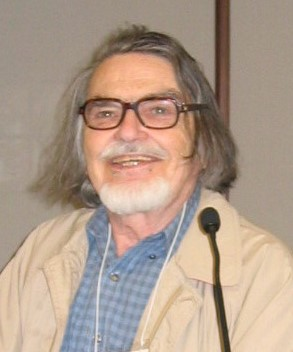
\includegraphics[scale=0.4]{img/Lambek.eps}
 \captionsetup{labelformat=empty}
 \caption{兰贝克(Joachim Lambek) 1922 - 2014}
 \label{fig:Lambek}
\end{figure}
%\end{wrapfigure}

\index{兰贝克定理}
1968年,兰贝克(Lambek)最早指出$i$是一个同构映射,并且称初始代数$(I, i)$是函子$\mathbf{F}$的不动点\cite{Lambek-1968}。现在这一事实被称作\textbf{兰贝克定理}。

F-代数中若存在初始代数$(I, i)$,则存在到任何其它代数$(A, f)$的唯一态射。我们把从$I$到$A$的态射记为$\lbb f \rbb$,使得下面的范畴图可交换:

\begin{center}
\begin{tikzpicture}
  \matrix (m) [matrix of math nodes,
               row sep=3em, column sep=3em, minimum width=2em]{
    \mathbf{F} I  & I \\
    \mathbf{F} A  & A \\};
  \path[-stealth]
    (m-1-1) edge node [above] {$i$} (m-1-2)
    (m-1-1) edge node [left] {$\mathbf{F} \lbb f \rbb$} (m-2-1)
    (m-1-2) edge node [right] {$\lbb f \rbb$}  (m-2-2)
    (m-2-1) edge node [below] {$f$} (m-2-2);
\end{tikzpicture}
\end{center}

\[
  \text{若} h = \lbb f \rbb \text{,当且仅当} h \circ i = f \circ \mathbf{F}(h)
\]

\index{向下态射(catamorphism)}
我们称箭头$\lbb f \rbb$为\textbf{向下态射}(catamorphism,来自希腊语$\kappa \alpha \kappa \alpha$,意思是向下)。它两侧的括号“$\lbb \rbb$”像一对香蕉,因此被称为“香蕉括号”。

向下态射的强大之处在于,它那能把一个非递归结构上的函数$f$,转换为在递归结构上的函数$\lbb f \rbb$。从而构造复杂的递归计算。我们仍然用自然数来举例子。

自然数函子$\mathbf{NatF}$是非递归的,而其起始代数自然数$\mathbf{Nat}$的定义是递归的:

\begin{lstlisting}
data NatF A = ZeroF | SuccF A

data Nat = Zero | Succ Nat
\end{lstlisting}

所以箭头$\mathbf{NatF} A \arrowto{f} A$是非递归的。一个$cata$(向下态射)能够从$f$构造出在递归的$\mathbf{Nat}$上进行计算的箭头$\mathbf{Nat} \to A$。所以$cata$的类型应为:

\[
(\mathbf{NatF} A \arrowto{f} A) \arrowto{cata} (\mathbf{Nat} \to A)
\]

所以(克里化的)$cata(f)$应该能够作用于$\mathbf{Nat}$的两种值$Zero$或者$Succ\ n$。我们可以根据这点定义出$cata$函数:

\[
\begin{array}{l}
cata\ f\ Zero = f\ ZeroF \\
cata\ f\ (Succ\ n) = f (SuccF\ (cata\ f\ n)) \\
\end{array}
\]

这一定义的第一行处理递归的边界情况。针对$\mathbf{Nat}$的零值$Zero$,我们转而用$f$对$\mathbf{NatF}A$的零值$Zero$求值;对于递归情况,也就是$\mathbf{Nat}$的值$Succ\ n$,我们先递归地用$cata\ f\ n$求出类型为$A$的值$a$,然后用$SuccF\ a$将其转化为$\mathbf{NatF}A$类型的值,最后再把$f$作用于其上。这个自然数的向下态射对于任何携带对象$A$都成立,它是非常通用的。我们进一步举两个具体的例子。第一个例子是将任何$\mathbf{Nat}$的值转换回$Int$。

\lstset{frame=single}
\begin{lstlisting}[style=Haskell]
toInt :: Nat -> Int
toInt = cata eval where
  eval :: NatF Int -> Int
  eval ZeroF = 0
  eval (SuccF x) = x + 1
\end{lstlisting}

这样$toInt\ Zero$会得到0,而$toInt\ (Succ\ (Succ\ (Succ\ Zero)))$会得到3。为了方便验证,可以再定义一个辅助函数:

\begin{lstlisting}[style=Haskell]
fromInt :: Int -> Nat
fromInt 0 = Zero
fromInt n = Succ (fromInt (n-1))
\end{lstlisting}

于任何整数$n$,有$n = (toInt \circ fromInt)\ n$。这个例子看起来很平常,我们来看第二个关于斐波那契数列的例子。

\begin{lstlisting}[style=Haskell]
toFib :: Nat -> (Integer, Integer)
toFib = cata fibAlg where
  fibAlg :: NatF (Integer, Integer) -> (Integer, Integer)
  fibAlg ZeroF = (1, 1)
  fibAlg (SuccF (m, n)) = (n, m + n)
\end{lstlisting}

我们特意将此前定义的函数$fib$改名为$fibAlg$,意思是说,从斐波那契的代数关系(非递归的),我们通过向下态射获得了递归计算斐波那契数列的能力。这样$toFib\ Zero$会得到数对$(1, 1)$,而$toFib\ (Succ\ (Succ\ (Succ\ Zero)))$会得到数对$(3, 5)$。下面的辅助函数,可以计算第$n$个斐波那契数。

\[
fibAt = fst \circ toFib \circ fromInt
\]

事实上,对于任何满足皮亚诺公理的类自然数代数结构$(A, c + f)$,我们都可以利用向下态射和初始代数$(\mathbf{Nat}, zero + succ)$,得到能够进行递归计算的$\lbb c + f \rbb$\footnote{我们用符号$\lbb c + f \rbb$是因为$\lbb [c, f] \rbb$看起来有太多重括号了。}。我们接下来证明这一点。考虑下面的范畴图。

\begin{center}
\begin{tikzpicture}
  \matrix (m) [matrix of math nodes,
               row sep=3em, column sep=5em, minimum width=2em]{
    \mathbf{NatF} \mathbf{Nat}  & \mathbf{Nat} \\
    \mathbf{NatF} A  & A \\};
  \path[-stealth]
    (m-1-1) edge node [above] {$[zero, succ]$} (m-1-2)
    (m-1-1) edge node [left] {$\mathbf{NatF}(h)$} (m-2-1)
    (m-1-2) edge node [right] {$h$}   (m-2-2)
    (m-2-1) edge node [below] {$[c, f]$} (m-2-2);
\end{tikzpicture}
\end{center}

由于向下态射使得这个范畴图可交换。

\[
\begin{array}{rll}
            & h \circ [zero, succ] = [c, f] \circ \mathbf{NatF}(h) & \text{可交换} \\
\Rightarrow & h \circ [zero, succ] = [c, f] \circ (id + h) & \text{多项式函子} \\
\Rightarrow & h \circ [zero, succ] = [c \circ id, f \circ h] & \text{右侧用余积的吸收律} \\
\Rightarrow & [h \circ zero, h \circ succ] = [c, f \circ h] & \text{左侧用余积的融合律} \\
\Rightarrow &
  \begin{cases}
    h \circ zero = c \\
    h \circ succ = f \circ h \\
  \end{cases} & \\
\Rightarrow &
  \begin{cases}
    h\ Zero = c \\
    h\ (Succ\ n) = f(h(n))
  \end{cases} & \\
\Rightarrow &
  \begin{cases}
    h(0) = c \\
    h(n + 1) = f(h(n))
  \end{cases} & \\
\end{array}
\]

这恰恰是自然数叠加的定义:

\[
  h = foldn(c, f)
\]

也就是说,自然数上的向下态射$\lbb c + f \rbb = foldn(c, f)$。因此,对于斐波那契数列,我们可以用

\[
\lbb fibAlg \rbb = \lbb start + next \rbb = foldn(start, next)
\]

来进行代数计算。读到这里,大家会有一种转了一大圈又回到了第一章的感觉。这是一种认知的螺旋上升。第一章中,我们是用归纳和抽象的方法得到了这个结论,现在,我们从更高的层面,把抽象的规律应用到具体的问题上得到了同样的结论。

\subsubsection{代数数据类型}

使用初始F-代数,我们可以定义更多的代数数据类型。本小节我们介绍列表和二叉树的例子。

\begin{example}
在第一章中,我们给出的列表定义为:

\lstset{frame=none}
\begin{lstlisting}
data List A = Nil | Cons A (List A)
\end{lstlisting}

而相应的非递归函子为:

\begin{lstlisting}
data ListF A B = NilF | ConsF A B
\end{lstlisting}

实际上$\mathbf{List}$是函子$\mathbf{ListF}$的不动点。我们可以这样验证。令$B' = \mathbf{ListF}\ A\ B$,然后递归地应用到自己上无穷多次。把这个结果叫做$\mathbf{Fix}\ (\mathbf{ListF}\ A)$:

\[
\begin{array}{rcll}
\mathbf{Fix}\ (\mathbf{ListF}\ A)
& = & \mathbf{ListF}\ A (\mathbf{Fix}\ (\mathbf{ListF}\ A)) & \text{不动点的定义} \\
& = & \mathbf{ListF}\ A\ (\mathbf{ListF}\ A\ (...)) & \text{展开} \\
& = & NilF\ |\ ConsF\ A\ (ConsF\ A\ (...)) & \text{定义} \\
& = & NilF\ |\ ConsF\ A\ (\mathbf{Fix}\ (\mathbf{ListF}\ A)) & \text{反向用不动点} \\
\end{array}
\]

和$\mathbf{List}\ A$的定义对比,我们有:

\[
\mathbf{List}\ A = \mathbf{Fix}\ (\mathbf{ListF}\ A)
\]

在$\mathbf{ListF}$这个函子下,固定$A$,对于任何携带对象$B$可以定义箭头

\[
\mathbf{ListF}\ A\ B \arrowto{f} B
\]

这样就构成了列表的F-代数。并且我们知道初始代数就是$(List, [nil, cons])$。所以就会有向下态射。

\begin{center}
\begin{tikzpicture}
  \matrix (m) [matrix of math nodes,
               row sep=3em, column sep=5em, minimum width=2em]{
    \mathbf{ListF}\ A\ (\mathbf{List}\ A)  & (\mathbf{List}\ A) \\
    \mathbf{ListF}\ A\ B & B \\};
  \path[-stealth]
    (m-1-1) edge node [above] {$[nil, cons]$} (m-1-2)
    (m-1-1) edge node [left] {$(\mathbf{ListF}\ A)(h)$} (m-2-1)
    (m-1-2) edge node [right] {$h$}   (m-2-2)
    (m-2-1) edge node [below] {$[c, f]$} (m-2-2);
\end{tikzpicture}
\end{center}

如果我们有一个非递归的计算$f$,就可以利用向下态射构成针对递归列表的计算。

\lstset{frame=single}
\begin{lstlisting}[style=Haskell]
cata :: (ListF a b -> b) -> (List a -> b)
cata f Nil = f NilF
cata f (Cons x xs) = f (ConsF x (cata f xs))
\end{lstlisting}

例如,可以定义计算列表长度的代数规则:

\begin{lstlisting}[style=Haskell]
len :: (List a) -> Int
len = cata lenAlg where
  lenAlg :: ListF a Int -> Int
  lenAlg NilF = 0
  lenAlg (ConsF _ n) = n + 1
\end{lstlisting}

这样$len\ Zero$会得到0,而$len\ (Cons\ 1\ (Cons\ 1\ Zero))$则得到2。可以定义一个辅助函数从中括弧简记法转换为$List$:

\begin{lstlisting}
fromList :: [a] -> List a
fromList [] = Nil
fromList (x:xs) = Cons x (fromList xs)
\end{lstlisting}

这样就可以通过$len (fromList [1, 1, 2, 3, 5, 8])$计算列表的长度。

通过改变代数规则$f$,还可以得到其它针对列表的计算。下面的例子把列表中所有的元素累加起来:

\begin{lstlisting}
sum :: (Num a) => (List a) -> a
sum = cata sumAlg where
  sumAlg :: (Num a) => ListF a a -> a
  sumAlg NilF = 0
  sumAlg (ConsF x y) = x + y
\end{lstlisting}

我们接下来利用列表的范畴图证明,列表的向下态射本质上就是叠加计算$foldr$。
列表函子本质上是多项式函子$\mathbf{ListF}\ A\ B = 1 + A \times B$。由于范畴图可交换,所以:

\[
\begin{array}{rll}
            & h \circ [nil, cons] = [c, f] \circ (\mathbf{ListF}\ A)(h) & \text{可交换} \\
\Rightarrow & h \circ [nil, cons] = [c, f] \circ (id + (id \times h)) & \text{多项式函子} \\
\Rightarrow & h \circ [nil, cons] = [c \circ id, f \circ (id \times h)] & \text{右侧用余积的吸收律} \\
\Rightarrow & [h \circ nil, h \circ cons] = [c, f \circ (id \times h)] & \text{左侧用余积的融合律} \\
\Rightarrow &
  \begin{cases}
    h \circ nil = c \\
    h \circ cons = f \circ (id \times h) \\
  \end{cases} & \\
\Rightarrow &
  \begin{cases}
    h\ Nil = c \\
    h\ (Cons\ a\ x) = f(a, h(x))
  \end{cases} & \\
\end{array}
\]

这恰恰是列表叠加的定义:

\[
  h = foldr(c, f)
\]

也就是说,列表F-代数的向下态射$\lbb c + f \rbb = foldr(c, f)$。因此,求长度的
运算是$foldr(0, (a, b) \mapsto b + 1)$,累加的运算是$foldr(0, +)$。
\end{example}

\begin{example}
在第二章中,我们定义了二叉树的类型为:

\lstset{frame=none}
\begin{lstlisting}
data Tree A = Nil | Br A (Tree A) (Tree A)
\end{lstlisting}

所有类似二叉树的结构也可以通过F-代数来描述。首先定义函子:

\begin{lstlisting}
data TreeF A B = NilF | BrF A B B
\end{lstlisting}

携带对象是$B$,而初始代数是$(\mathbf{Tree}\ A, [nil, branch])$。我们把证明作为本小节的练习。这样二叉树的向下态射表示为如下范畴图:

\begin{center}
\begin{tikzpicture}
  \matrix (m) [matrix of math nodes,
               row sep=3em, column sep=5em, minimum width=2em]{
    \mathbf{TreeF}\ A\ (\mathbf{Tree}\ A)  & (\mathbf{Tree}\ A) \\
    \mathbf{TreeF}\ A\ B & B \\};
  \path[-stealth]
    (m-1-1) edge node [above] {$[nil, branch]$} (m-1-2)
    (m-1-1) edge node [left] {$(\mathbf{TreeF}\ A)(h)$} (m-2-1)
    (m-1-2) edge node [right] {$h$}   (m-2-2)
    (m-2-1) edge node [below] {$[c, f]$} (m-2-2);
\end{tikzpicture}
\end{center}

我们可以定义二叉树的向下态射函数。它接受一个F-代数的箭头$\mathbf{TreeF}\ A\ B \arrowto{f} B$,返回一个从$\mathbf{Tree}\ A \to B$的函数:

\[
\begin{array}{l}
cata : (\mathbf{TreeF}\ A\ B \to B) \to (\mathbf{Tree}\ A \to B) \\
cata\ f\ Nil = f\ NilF \\
cata\ f\ (Br\ k\ l\ r) =f\ (BrF\ k\ (cata\ f\ l)\ (cata\ f\ r)) \\
\end{array}
\]

如果定义了一个将二叉树中元素累加起来的代数运算,就可以利用向下态射递归地应用到任意二叉树上:

\[
\begin{array}{l}
sum : \mathbf{Tree}\ A \to A \\
sum = cata \circ sumAlg \\
\text{其中:}
      \begin{cases}
        sumAlg : \mathbf{TreeF}\ A\ B \to B \\
        sumAlg\ NilF = 0_{B} \\
        sumAlg\ (Br\ k\ l\ r) = k + l + r \\
      \end{cases} \\
\end{array}
\]

接下来,我们证明二叉树的向下态射就相当于二叉树的叠加操作$foldt$。固定对象$A$,二叉树的函子$\mathbf{TreeF}\ A\ B$是携带对象$B$的一个多项式函子。即:$\mathbf{TreeF}\ A\ B = 1 + (A \times B \times B)$,对于箭头$h$,为:$(\mathbf{TreeF}\ A)(h) = id + (id_A \times h \times h)$。

由于上面的范畴图可交换,所以有:

\[
\begin{array}{rll}
            & h \circ [nil, branch] = [c, f] \circ (\mathbf{TreeF}\ A)(h) & \text{可交换} \\
\Rightarrow & h \circ [nil, branch] = [c, f] \circ (id + (id_A \times h \times h)) & \text{多项式函子} \\
\Rightarrow & h \circ [nil, branch] = [c \circ id, f \circ (id_A \times h \times h)] & \text{右侧用余积的吸收律} \\
\Rightarrow & [h \circ nil, h \circ branch] = [c, f \circ (id_A \times h)] & \text{左侧用余积的融合律} \\
\Rightarrow &
  \begin{cases}
    h \circ nil = c \\
    h \circ branch = f \circ (id_A \times h \times h) \\
  \end{cases} & \\
\Rightarrow &
  \begin{cases}
    h\ Nil = c \\
    h\ (Br\ k\ l\ r) = f(k, h(l), h(r))
  \end{cases} & \\
\end{array}
\]

这恰恰是二叉树叠加的定义$h = foldt(c, f)$,其中:

\[
\begin{cases}
foldt\ c\ h\ Nil = c \\
foldt\ c\ h\ (Br\ k\ l\ r) = h(k, foldt\ c\ h\ l, foldt\ c\ h\ r) \\
\end{cases}
\]

因此,累加二叉树中元素的运算可以用叠加表示为$foldt(0_B, (\bullet + \bullet + \bullet))$。
\end{example}

\begin{Exercise}
\Question{对二叉树函子$\mathbf{TreeF}\ A\ B$,固定$A$,利用不动点验证$(\mathbf{Tree}\ A, [nil, branch])$是初始代数。}
\end{Exercise}

\section{小节}

本章介绍了范畴论中最基本的概念,包括范畴、函子、自然变换。并且还介绍了积和余积、起始对象和终止对象、幂以及F-代数这些工具来构造较为复杂的代数结构。作为本章的结尾,我们来解读最开始那段关于叠加的代码\cite{Haskell-foldable}:

\lstset{frame=single}
\begin{lstlisting}
foldr f z t = appEndo (foldMap (Endo . f) t) z
\end{lstlisting}

所有的这一切的背后都是为了抽象,为了使得$foldr$能跳出列表,在任何可叠加的结构上进行运算。我们先看看传统的列表叠加定义:

\begin{lstlisting}
foldr :: (a -> b -> b) -> b -> [a] -> b
foldr f z [] = z
foldr f z (x:xs) = f x (foldr f z xs)
\end{lstlisting}

其中$f$是一个二元操作,如果我们把它改写为$\oplus$,把$z$改写为单位元$e$,根据这个定义,$foldr\ (\oplus)\ e\ [a, b, c]$就可以展开成为:

\[
a \oplus (b \oplus (c \oplus e))
\]

这让我们联想到幺半群,$foldr$相当于在幺半群上重复进行二元操作。在Haskell的抽象幺半群定义中,除了单位元和二元操作外,还定义了将一列元素“累加”的操作。用我们的$\oplus$和$e$符号,这个定义相当于:

\[
\begin{array}{l}
concat_M : [M] \to M \\
concat_M = foldr\ (\oplus)\ e \\
\end{array}
\]

在Haskell中这个函数的名字叫做\texttt{mconcat}。它的意思是说,对于任何幺半群$M$,$concat$可以将一个$M$中元素的列表,通过二元运算和单位元叠加计算到一起。例如字符串可以看作是幺半群,单位元是空串,而二元运算是连接。所以$concat_M$ \texttt{["Hello", "String" "Monoid"]}就得到:

\begin{verbatim}
"Hello" ++ ("String" ++ ("Monoid" ++ "")) = "HelloStringMonoid"
\end{verbatim}

现在我们可以对任何幺半群元素进行累加了。但能否让它变得更通用呢?如果有一列元素,它们虽然不是幺半群中的元素,但是如果我们能将它们转换为幺半群,就仍然可以进行累加。将某一类型的列表映射为幺半群列表恰巧就是函子的行为,确切地说我们把箭头$A \arrowto{g} M$,通过列表函子“举”到$\mathbf{List}(g)$。然后再执行累加:

\begin{center}
\begin{tikzpicture}
  \matrix (m) [matrix of math nodes,
               row sep=2em, column sep=5em, minimum width=2em]{
     \lbrack A \rbrack & \lbrack M \rbrack & M\\
     A   &  M  & \\};
  \path[-stealth]
    (m-1-1) edge node [above] {$fmap\ g$} (m-1-2)
    (m-2-1) edge node [above] {$g$} (m-2-2)
    (m-2-1) edge node [left] {$\mathbf{List}$} (m-1-1)
    (m-2-2) edge node [right] {$\mathbf{List}$} (m-1-2)
    (m-1-2) edge node [above] {$concat$} (m-1-3);
\end{tikzpicture}
\end{center}

\[
\begin{array}{l}
foldMap : (A \to M) \to [A] \to M \\
foldMap\ g = concat_M \circ fmap\ g
\end{array}
\]

可是美中不足的是,对于任何传入$foldr$的二元组合函数$f : A \to B \to B$,如果$B$不是幺半群,我们仍然无法进行叠加。现在考虑$f$的克里化形式$f : A \to (B \to B)$,我们发现以箭头$B \to B$为对象,可以组成一个幺半群。其中单位元是恒等箭头$id$,而二元运算是函数组合。为此,我们把这种$B \to B$的箭头通过函子封装成一个类型(集合):

\lstset{frame=none}
\begin{lstlisting}[style=Haskell]
newtype Endo B = Endo (B -> B)
\end{lstlisting}

并且定义一个函数,从$\mathbf{Endo}B \arrowto{appEndo} B$:

\[
appEndo(Endo\ a) = a
\]

然后我们规定$\mathbf{Endo}$是一个幺半群,单位元是$id$,二元运算是函数组合。在Haskell中,这相当于以下代码:

\lstset{frame=single}
\begin{lstlisting}[style=Haskell]
instance Monoid Endo where
    mempty = Endo id
    Endo f `mappend` Endo g = Endo (f . g)
\end{lstlisting}

现在任给一个二元组合函数$f$,我们都可以把它利用$foldMap$叠加到$Endo$幺半群上去了:

\[
\begin{array}{l}
foldCompose : (A \to (B \to B)) \to [A] \to \mathbf{Endo}B \\
foldCompose\ f = foldMap\ (Endo . f)
\end{array}
\]

这样如果计算$foldCompose\ f\ [a, b, c]$则展开为:

\[
\begin{array}{cl}
  & Endo(f\ a) \oplus (Endo(f\ b) \oplus (Endo(f\ c) \oplus Endo(id))) \\
= & Endo(f\ a \oplus (f\ b \oplus (f\ c \oplus id))
\end{array}
\]

下面是一个具体的例子

\[
\begin{array}{cl}
            & foldCompose\ (+)\ [1, 2, 3] \\
\Rightarrow & foldMap\ (Endo \circ (+))\ [1, 2, 3] \\
\Rightarrow & concat_M\ (fmap (Endo \circ (+)))\ [1, 2, 3] \\
\Rightarrow & concat_M\ (fmap Endo\ [(+1), (+2), (+3)]) \\
\Rightarrow & concat_M\ [Endo\ (+1), Endo\ (+2), Endo\ (+3)] \\
\Rightarrow & Endo\ ((+1) \circ (+2) \circ (+3)) \\
\Rightarrow & Endo\ (+6) \\
\end{array}
\]

所以,最后一步我们要把$Endo$中的结果取回。具体到这个例子,就是用$appEndo$把$(+6)$拿出,然后把它应用到传入$foldr$的初始值$z$上:

\[
\begin{array}{rcll}
foldr\ f\ z\ xs
  & = & appEndo\ (foldCompose\ f\ xs)\ z & \\
  & = & appEndo\ (foldMap\ (Endo \circ f)\ xs)\ z \\
\end{array}
\]

这就是我们在本章开头给出的$foldr$定义。在Haskell中,还专门定义了类型$Foldable$,对任意数据结构,使用者可以选择实现$foldMap$或者$foldr$。具体请参见本章附录。

\section{扩展阅读}

限于篇幅,我们不可能仅仅在一章中完成范畴论的介绍。本章的内容不过是冰山的一个小角。范畴论的核心精神是抽象。初始对象和终止对象,积和余积这些对偶的概念,它们本质上可以进一步抽象到更高层次的对偶——极限(limits)和余极限(colimits)。我们没能介绍伴随(junction)的概念,没能介绍米田定理(Yoneda lemma),也没有能够解读单子。我希望这一章能够起到抛砖引玉的作用,引导读者去阅读和了解更多的内容。范畴论的创始人之一麦克兰恩的编写的教材\cite{Mac-Lane-1998}是这个领域的经典。其目标读者是数学家,普通读者读起来有些艰深。西蒙森的《范畴论引论》\cite{Simmons2011}和史密斯的\cite{PeterSmith2018}更适合初学者。对于有编程背景的读者,迈尔维斯基的《程序员的范畴论》\cite{Milewski2018}是本不错的参考书。里面配有很多Haskell示例代码和一些C++的类比实现。但是这本书仅仅在集合全函数范畴(确切地说是Hask范畴)内讨论。伯德的《编程中的代数》\cite{Bird97}更加全面地介绍了编程中的范畴原理。

% limits/colimits, 伴随,米田定理

\section{附录:例子代码}

函子的定义:

\lstset{frame=single}
\begin{lstlisting}[style=Haskell]
class  Functor f  where
    fmap        :: (a -> b) -> f a -> f b
\end{lstlisting}

Maybe函子的定义:

\begin{lstlisting}
instance  Functor Maybe  where
    fmap _ Nothing       = Nothing
    fmap f (Just a)      = Just (f a)
\end{lstlisting}

使用Maybe搜索二叉搜索树,并将结果转换成二进制:

\begin{lstlisting}[style=Haskell]
lookup Nil _ = Nothing
lookup (Node l k r) x | x < k = lookup l x
                      | x > k = lookup r x
                      | otherwise = Just k

lookupBin = (fmap binary) . lookup
\end{lstlisting}

二元函子的定义:

\begin{lstlisting}
class Bifunctor f where
  bimap :: (a -> c) -> (b -> d) -> f a b -> f c d
\end{lstlisting}

积函子和余积函子的定义:

\begin{lstlisting}
instance Bifunctor (,) where
  bimap f g (x, y) = (f x, g y)

instance Bifunctor Either where
  bimap f _ (Left a) = Left (f a)
  bimap _ g (Right b) = Right (g b)
\end{lstlisting}

$curry$及其反向变换$uncurry$的定义:

\begin{lstlisting}
curry       :: ((a, b) -> c) -> a -> b -> c
curry f x y =  f (x, y)

uncurry     :: (a -> b -> c) -> ((a, b) -> c)
uncurry f (x, y) =  f x y
\end{lstlisting}

幺半群的定义:

\begin{lstlisting}
class Semigroup a => Monoid a where
    mempty  :: a

    mappend :: a -> a -> a
    mappend = (<>)

    mconcat :: [a] -> a
    mconcat = foldr mappend mempty
\end{lstlisting}

可叠加类型(Foldable)的定义:

\begin{lstlisting}
newtype Endo a = Endo { appEndo :: a -> a }

class Foldable t where
    foldr :: (a -> b -> b) -> b -> t a -> b
    foldr f z t = appEndo (foldMap (Endo . f) t) z

    foldMap :: Monoid m => (a -> m) -> t a -> m
    foldMap f = foldr (mappend . f) mempty
\end{lstlisting}

\ifx\wholebook\relax \else
\begin{thebibliography}{99}

\bibitem{Dieudonne1987}
Jean Dieudonne. ``Mathematics — The Music of Reason''. Springer Science and Business Media, Jul 20, 1998. ISBN: 9783540533467

\bibitem{Monad-Haskell-Wiki}
Haskell Wiki. ``Monad''. \url{https://wiki.haskell.org/Monad}

\bibitem{Wiki-Eilenberg}
Wikipedia. ``塞缪尔$\cdot$艾伦伯格''. \url{https://en.wikipedia.org/wiki/Samuel_Eilenberg}

\bibitem{Wiki-Mac-Lane}
Wikipedia. ``桑德斯$\cdot$麦克兰恩''. \url{https://en.wikipedia.org/wiki/Saunders_Mac_Lane}

\bibitem{Simmons2011}
Harold Simmons. ``An introduction to Category Theory''.  Cambridge University Press; 1 edition, 2011. ISBN: 9780521283045

\bibitem{Wiki-Hoare}
Wikipedia. ``Tony Hoare''. \url{https://en.wikipedia.org/wiki/Tony_Hoare}

\bibitem{Wadler-1989}
Wadler Philip. ``Theorems for free!''. Functional Programming Languages and Computer Architecture, pp. 347-359. Asociation for Computing Machinery. 1989.

\bibitem{Milewski2018}
Bartosz Milewski. ``Category Theory for Programmers''. \url{https://bartoszmilewski.com/2014/10/28/category-theory-for-programmers-the-preface/}

\bibitem{Bird97}
Richard Bird, Oege de Moor. ``Algebra of Programming''. University of Oxford, Prentice Hall Europe. 1997. ISBN: 0-13-507245-X.

\bibitem{PeterSmith2018}
Peter Smith. ``Category Theory - A Gentle Introduction''. \url{http://www.academia.edu/21694792/A_Gentle_Introduction_to_Category_Theory_Jan_2018_version_}

\bibitem{Wiki-Exponentials}
Wikipedia. ``Exponential Object''. \url{https://en.wikipedia.org/wiki/Exponential_object}

\bibitem{Manes-Arbib-1986}
Manes, E. G. and Arbib, M. A. ``Algebraic Approaches to Program Semantics''. Texts and Monographs in Computer Science. Springer-Verlag. 1986.

\bibitem{Lambek-1968}
Lambek, J. ``A fixpoint theorem for complete categories''. Mathematische Zeischrift, 103, pp.151-161. 1968.

\bibitem{Haskell-foldable}
Wikibooks. ``Haskell/Foldable''.  \url{https://en.wikibooks.org/wiki/Haskell/Foldable}

\bibitem{Mac-Lane-1998}
Mac Lane. ``Categories for working mathematicians''. Springer-Verlag. 1998. ISBN: 0387984038.

\end{thebibliography}

\expandafter\enddocument
%\end{document}

\fi
